\documentclass[a4paper, 12pt]{article}
\usepackage{amsmath}
\usepackage{amsfonts}
\usepackage{setspace}
\usepackage{hyperref}
\usepackage{mathrsfs}
\usepackage{graphicx}
\usepackage[utf8]{inputenc}
\usepackage{tcolorbox}
\usepackage{caption}
 \usepackage{multirow}
 \usepackage{float}
 \restylefloat{table}
 \usepackage{imakeidx}
\usepackage{subfigure}
\usepackage{adjustbox}
\usepackage{courier}
\usepackage{mathtools}
\usepackage[toc,page]{appendix}
\usepackage[square, numbers]{natbib}
\graphicspath{ {figures/} }
\usepackage{array}

\usepackage[a4paper,margin=1.5in]{geometry}

% adding list of symbols
\usepackage{glossaries}
\makeglossaries
\newglossaryentry{rel_velocity}{
	name=\ensuremath{\Delta v},
	description={Relative velocity [km/s]}
}
\newglossaryentry{flux}{
	name=\ensuremath{\Phi},
	description={Flux of fragments}
}
\newglossaryentry{mean}{
	name=\ensuremath{\mu},
	description={Mean value}
}
\newglossaryentry{grav_param_E}{
	name=\ensuremath{\mu_E},
	description={Earth's planetary gravitational constant [km3/ s2]}
}
\newglossaryentry{true_anomaly}{
	name=\ensuremath{\nu},
	description={True anomaly [rad or deg]}
}
\newglossaryentry{raan}{
	name=\ensuremath{\Omega},
	description={Longitude of the ascending node [rad or deg]}
}
\newglossaryentry{argp}{
	name=\ensuremath{\omega},
	description={Argument of the periapsis [rad or deg]}
}
\newglossaryentry{density}{
	name=\ensuremath{\rho},
	description={Atmosphere density [kg / m3]}
}
\newglossaryentry{area}{
	name=\ensuremath{A},
	description={Cross-sectional area [m2]}
}
\newglossaryentry{semi_major_axis}{
	name=\ensuremath{a},
	description={Semi-major axis [km]}
}
\newglossaryentry{eccentricity}{
	name=\ensuremath{e},
	description={Eccentricity}
}
\newglossaryentry{scale_height}{
	name=\ensuremath{H},
	description={Scale height for exponential atmospheric model [km]}
}
\newglossaryentry{altitude}{
	name=\ensuremath{h},
	description={Altitude [km]}
}
\newglossaryentry{inclination}{
	name=\ensuremath{i},
	description={Inclination [rad or deg]}
}
\newglossaryentry{bessel}{
	name=\ensuremath{I_k},
	description={Modified Bessel function of the first kind and order k }
}
\newglossaryentry{J2}{
	name=\ensuremath{J_2},
	description={Second zonal harmonic coefficient for the Earth }
}
\newglossaryentry{L_c}{
	name=\ensuremath{L_c},
	description={Fragment characteristic length [m] }
}
\newglossaryentry{mass}{
	name=\ensuremath{M},
	description={Mass [kg] }
}
\newglossaryentry{reference_mass}{
	name=\ensuremath{M_e},
	description={Reference mass for collisions[kg] }
}
\newglossaryentry{prjectile_mass}{
	name=\ensuremath{M_p},
	description={Projectile mass[kg] }
}
\newglossaryentry{target_mass}{
	name=\ensuremath{M_t},
	description={Target mass[kg] }
}
\newglossaryentry{normal_distribution}{
	name=\ensuremath{\mathcal{N}},
	description={Normal distribution }
}
\newglossaryentry{impact_vel}{
	name=\ensuremath{v_c},
	description={Relative impact velocity [km/s] }
}

% Matrix stretching
\renewcommand{\arraystretch}{0.5} % because \baselinestretch is 1.6667

% Default fixed font does not support bold face
\DeclareFixedFont{\ttb}{T1}{txtt}{bx}{n}{12} % for bold
\DeclareFixedFont{\ttm}{T1}{txtt}{m}{n}{12}  % for normal


% Custom colors
\usepackage{color}
\definecolor{deepblue}{rgb}{0,0,0.5}
\definecolor{deepred}{rgb}{0.6,0,0}
\definecolor{deepgreen}{rgb}{0,0.5,0}

\usepackage{listings, lstautogobble}

\graphicspath{ {figures/} }

\tcbuselibrary{minted,breakable,xparse,skins}
\newenvironment{code}{\captionsetup{type=listing}}{}
\definecolor{bg}{gray}{1}
\DeclareTCBListing{mintedbox}{O{}m!O{}}{%
	breakable=true,
	listing engine=minted,
	listing only,
	minted language=#2,
	minted style=default,
	minted options={%
		linenos,
		gobble=0,
		breaklines=true,
		breakafter=,,
		fontsize=\small,
		numbersep=8pt,
		#1},
	boxsep=0pt,
	left skip=0pt,
	right skip=0pt,
	left=25pt,
	right=0pt,
	top=3pt,
	bottom=3pt,
	arc=5pt,
	leftrule=0pt,
	rightrule=0pt,
	bottomrule=2pt,
	toprule=2pt,
	colback=bg,
	colframe=gray!70,
	enhanced,
	overlay={%
		\begin{tcbclipinterior}
			\fill[gray!20!white] (frame.south west) rectangle ([xshift=20pt]frame.north west);
	\end{tcbclipinterior}},
	#3}

\newtcblisting{tcbpythoncode}[1][python]{%
	colback         = gray!5        ,
	colframe        = gray!50!black ,
	listing only                      ,
	title           = #1              ,
	halign title    = right           ,
	fonttitle       = \bfseries       ,
	listing engine  = minted          ,
	minted language = python
}


% NEWEST CODE FOFRMTATTING

\lstloadlanguages{ 
	Python
}
\usepackage{xcolor}
\definecolor{maroon}{cmyk}{0, 0.87, 0.68, 0.32}
\definecolor{halfgray}{gray}{0.55}
\definecolor{ipython_frame}{RGB}{207, 207, 207}
\definecolor{ipython_bg}{RGB}{247, 247, 247}
\definecolor{ipython_red}{RGB}{186, 33, 33}
\definecolor{ipython_green}{RGB}{0, 128, 0}
\definecolor{ipython_cyan}{RGB}{64, 128, 128}
\definecolor{ipython_purple}{RGB}{170, 34, 255}
\lstdefinelanguage{iPython}{
	morekeywords={access,and,break,class,continue,def,del,elif,else,except,exec,finally,for,from,global,if,import,in,is,lambda,not,or,pass,print,raise,return,try,while},%
	%
	% Built-ins
	morekeywords=[2]{abs,all,any,basestring,bin,bool,bytearray,callable,chr,classmethod,cmp,compile,complex,delattr,dict,dir,divmod,enumerate,eval,execfile,file,filter,float,format,frozenset,getattr,globals,hasattr,hash,help,hex,id,input,int,isinstance,issubclass,iter,len,list,locals,long,map,max,memoryview,min,next,object,oct,open,ord,pow,property,range,raw_input,reduce,reload,repr,reversed,round,set,setattr,slice,sorted,staticmethod,str,sum,super,tuple,type,unichr,unicode,vars,xrange,zip,apply,buffer,coerce,intern},%
	%
	sensitive=true,%
	morecomment=[l]\#,%
	morestring=[b]',%
	morestring=[b]",%
	%
	morestring=[s]{'''}{'''},% used for documentation text (mulitiline strings)
	morestring=[s]{"""}{"""},% added by Philipp Matthias Hahn
	%
	morestring=[s]{r'}{'},% `raw' strings
	morestring=[s]{r"}{"},%
	morestring=[s]{r'''}{'''},%
	morestring=[s]{r"""}{"""},%
	morestring=[s]{u'}{'},% unicode strings
	morestring=[s]{u"}{"},%
	morestring=[s]{u'''}{'''},%
	morestring=[s]{u"""}{"""},%
	%
	% {replace}{replacement}{lenght of replace}
	% *{-}{-}{1} will not replace in comments and so on
	literate=
	{á}{{\'a}}1 {é}{{\'e}}1 {í}{{\'i}}1 {ó}{{\'o}}1 {ú}{{\'u}}1
	{Á}{{\'A}}1 {É}{{\'E}}1 {Í}{{\'I}}1 {Ó}{{\'O}}1 {Ú}{{\'U}}1
	{à}{{\`a}}1 {è}{{\`e}}1 {ì}{{\`i}}1 {ò}{{\`o}}1 {ù}{{\`u}}1
	{À}{{\`A}}1 {È}{{\'E}}1 {Ì}{{\`I}}1 {Ò}{{\`O}}1 {Ù}{{\`U}}1
	{ä}{{\"a}}1 {ë}{{\"e}}1 {ï}{{\"i}}1 {ö}{{\"o}}1 {ü}{{\"u}}1
	{Ä}{{\"A}}1 {Ë}{{\"E}}1 {Ï}{{\"I}}1 {Ö}{{\"O}}1 {Ü}{{\"U}}1
	{â}{{\^a}}1 {ê}{{\^e}}1 {î}{{\^i}}1 {ô}{{\^o}}1 {û}{{\^u}}1
	{Â}{{\^A}}1 {Ê}{{\^E}}1 {Î}{{\^I}}1 {Ô}{{\^O}}1 {Û}{{\^U}}1
	{œ}{{\oe}}1 {Œ}{{\OE}}1 {æ}{{\ae}}1 {Æ}{{\AE}}1 {ß}{{\ss}}1
	{ç}{{\c c}}1 {Ç}{{\c C}}1 {ø}{{\o}}1 {å}{{\r a}}1 {Å}{{\r A}}1
	{€}{{\EUR}}1 {£}{{\pounds}}1
	%
	{^}{{{\color{ipython_purple}\^{}}}}1
	{=}{{{\color{ipython_purple}=}}}1
	%
	{+}{{{\color{ipython_purple}+}}}1
	{*}{{{\color{ipython_purple}$^\ast$}}}1
	{/}{{{\color{ipython_purple}/}}}1
	%
	{+=}{{{+=}}}1
	{-=}{{{-=}}}1
	{*=}{{{$^\ast$=}}}1
	{/=}{{{/=}}}1,
	literate=
	*{-}{{{\color{ipython_purple}-}}}1
	{?}{{{\color{ipython_purple}?}}}1,
	%
	identifierstyle=\color{black}\ttfamily,
	commentstyle=\color{ipython_cyan}\ttfamily,
	stringstyle=\color{ipython_red}\ttfamily,
	keepspaces=true,
	showspaces=false,
	showstringspaces=false,
	%
	rulecolor=\color{ipython_frame},
	frame=single,
	frameround={t}{t}{t}{t},
	framexleftmargin=6mm,
	numbers=left,
	numberstyle=\tiny\color{halfgray},
	%
	%
	backgroundcolor=\color{ipython_bg},
	%   extendedchars=true,
	basicstyle=\scriptsize,
	keywordstyle=\color{ipython_green}\ttfamily,
}

\lstset{
	basicstyle=\ttm, % Default font
	numbers=left,              % Location of line numbers
	numberstyle=\tiny,          % Style of line numbers
	stepnumber=1,              % Margin between line numbers
	numbersep=5pt,              % Margin between line numbers and text
	tabsize=2,                  % Size of tabs
	extendedchars=true,
	breaklines=true,            % Lines will be wrapped
	keywordstyle=\color{red},
	frame=b,
	% keywordstyle=[1]\textbf,
	% keywordstyle=[2]\textbf,
	% keywordstyle=[3]\textbf,
	% keywordstyle=[4]\textbf,   \sqrt{\sqrt{}}
	stringstyle=\color{white}\ttfamily, % Color of strings
	showspaces=false,
	showtabs=false,
	xleftmargin=17pt,
	framexleftmargin=17pt,
	framexrightmargin=5pt,
	framexbottommargin=4pt,
	% backgroundcolor=\color{lightgray},
	showstringspaces=false,
	autogobble=true,
	morekeywords={self},
	language=iPython,
	literate=
	{á}{{\'a}}1 {é}{{\'e}}1 {í}{{\'i}}1 {ó}{{\'o}}1 {ú}{{\'u}}1
	{Á}{{\'A}}1 {É}{{\'E}}1 {Í}{{\'I}}1 {Ó}{{\'O}}1 {Ú}{{\'U}}1
	{à}{{\`a}}1 {è}{{\`e}}1 {ì}{{\`i}}1 {ò}{{\`o}}1 {ù}{{\`u}}1
	{À}{{\`A}}1 {È}{{\'E}}1 {Ì}{{\`I}}1 {Ò}{{\`O}}1 {Ù}{{\`U}}1
	{ä}{{\"a}}1 {ë}{{\"e}}1 {ï}{{\"i}}1 {ö}{{\"o}}1 {ü}{{\"u}}1
	{Ä}{{\"A}}1 {Ë}{{\"E}}1 {Ï}{{\"I}}1 {Ö}{{\"O}}1 {Ü}{{\"U}}1
	{â}{{\^a}}1 {ê}{{\^e}}1 {î}{{\^i}}1 {ô}{{\^o}}1 {û}{{\^u}}1
	{Â}{{\^A}}1 {Ê}{{\^E}}1 {Î}{{\^I}}1 {Ô}{{\^O}}1 {Û}{{\^U}}1
	{œ}{{\oe}}1 {Œ}{{\OE}}1 {æ}{{\ae}}1 {Æ}{{\AE}}1 {ß}{{\ss}}1
	{ç}{{\c c}}1 {Ç}{{\c C}}1 {ø}{{\o}}1 {å}{{\r a}}1 {Å}{{\r A}}1
	{€}{{\EUR}}1 {£}{{\pounds}}1
}
\DeclareCaptionFont{white}{\color{white}}
\DeclareCaptionFormat{listing}{\colorbox[cmyk]{0.43, 0.35, 0.35,0.01}{\parbox{\textwidth}{\hspace{15pt}#1#2#3}}}
\captionsetup[lstlisting]{format=listing,labelfont=white,textfont=white, singlelinecheck=false, margin=0pt, font={bf,footnotesize}}


\makeatletter
\renewcommand\section{\clearpage\newpage\@startsection {section}{1}{\z@}%
	{-3.5ex \@plus -1ex \@minus -.2ex}%
	{2.3ex \@plus.2ex}%
	{\normalfont\Large\bfseries}}
\makeatother


% Index code
\makeindex

\newcommand{\lindex}[1]{%
	\lowercase{\def\temp{#1}}%
	\expandafter\index\expandafter{\temp}%
}

\newcommand{\boldindex}[1]{%
	\textbf{#1}\lindex{#1}%
}

\renewcommand{\thefigure}{\arabic{section}.\arabic{figure}}


% Math eqn sizing
\addtolength{\jot}{1em} % Spacing betwn align



\begin{document}

%==========================================================================
%==========================================================================
% Title pages.

\newcommand\ddfrac[2]{\frac{\displaystyle #1}{\displaystyle #2}}
\newcommand{\mytitle}{Orbital Debris Cloud Evolution: An analysis of fragmentation events in low earth orbit}
\newcommand{\myauthor}{Reece Humphreys}
\newcommand{\myadvisor}{Dr. Yaouen Fily}

\newcommand{\myskip}{\vspace{0.5in}}
\newcommand{\layouttitle}[1]{{\bf\large\MakeUppercase{#1}}}
\setlength{\parindent}{0em}
\doublespacing
\renewcommand{\arraystretch}{0.6} % because \baselinestretch is 1.6667
\pagenumbering{roman}
\thispagestyle{empty}

\begin{center}

	\vspace{4in} 
	\layouttitle{\mytitle} \\ by \\ \myauthor
	
	\vspace{1in}
	A Thesis Submitted to the Faculty of \\
	The Wilkes Honors College \\
	in Partial Fulfillment of the Requirements for the Degree of \\
	Bachelor of Science in Liberal Arts and Sciences \\
	with a Concentration in Physics \\ 
	\vspace{1in} 
	Wilkes Honors College of \\
	Florida Atlantic University \\
	Jupiter, Florida \\
	May \number\year

\end{center}

\newpage

%==========================================================================

\vspace{4in}
\begin{center}
	\layouttitle{\mytitle} \\
	by \\
	\myauthor
\end{center}

\singlespace
\vspace{1in}
This thesis was prepared under the direction of the candidate's thesis advisor, \myadvisor, and has been approved by the members of their supervisory committee. It was submitted to the faculty of the Harriet L. Wilkes Honors College and was accepted in partial fulfillment of the requirements for the degree of Bachelor of Science in Liberal Arts and Sciences.

\vspace{1in}
SUPERVISORY COMMITTEE:

\newcommand{\myrule}{\vspace{0.5in}\rule{4in}{0.5pt} \\}

\myrule
\myadvisor

\myrule 
{}[second reader]

\myrule
Interim Dean Timothy Steigenga, Harriet L. Wilkes Honors College 

\myrule
Date

\newpage

%==========================================================================

%\begin{center}
%	\layouttitle{Acknowledgements}
%\end{center}
%\section*{Acknowledgments}
%\addcontentsline{toc}{section}{Acknowledgements}

\myskip
%Some acknowledgments.

\newpage

%==========================================================================

%\begin{center}
%	\layouttitle{Abstract}
%\end{center}
\section*{Abstract}
\addcontentsline{toc}{section}{Abstract}

\myskip
\renewcommand{\arraystretch}{1.5}
\begin{tabular}{@{}l@{\hspace{3ex}}l}
	Author: & \myauthor \\
	Title: & Orbital Debris Cloud Evolution: An analysis \\
	 & of fragmentation events in low Earth orbit \\
	Institution: & Harriet L. Wilkes Honors College, Florida Atlantic  \\
	& University \\
	Thesis Advisor: & \myadvisor \\
	Degree: & Bachelor of Science in Liberal Arts and Sciences \\
	Concentration: & Mathematics \\
	Year: & \the\year
\end{tabular}


\myskip
\doublespace
Orbital debris has quickly become one of the newest sources of pollution as a result of mankind's desire to work in, explore, and utilize space. However, unlike most types of pollution which people experience daily, this is pollution that is impossible for the average person to ever encounter. Yet they poses just as grand of a threat as the other types. Orbital debris is the remnants of orbital collisions, weapons tests, decommissioned satellites, and spent rocket stages that are passing over our heads faster than bullets and containing similar energy to hand grenades. This paper explores the existing models of orbital debris generation, how clouds of debris evolve with respect to time, and the ramifications that they pose.
\singlespace
\newpage

%==========================================================================

\tableofcontents

\cleardoublepage
\addcontentsline{toc}{section}{\listfigurename}\listoffigures

\cleardoublepage
\addcontentsline{toc}{section}{\listtablename}\listoftables

\glsaddall
\cleardoublepage
\addcontentsline{toc}{section}{List of Symbols}\printglossary[title={List of Symbols}, nonumberlist]

%==========================================================================
\newpage
\setlength{\parindent}{1em}
\pagenumbering{arabic}

%==========================================================================
%==========================================================================
% Thesis proper.


\section{Introduction}
\label{introduction}
\doublespace
\subsection{Motivation}
Due to the accelerating launch cadence in the space sector, increased accessibility and resources for small teams to create cube satellites, and satellite mega constellation constructions underway, researchers have become increasingly concerned about the implications of potential orbital collisions. These worries have been compounded by the actions taken by foreign nations with regards to anti-satellite weapons which create substantial amounts of debris. In one such instance, a 2007 Chinese anti-satellite missile test was universally condemned and received statements from government officials such as the U.K. prime minister whose spokesperson stated, ``We are concerned about the impact of debris in space and we expressed that concern.'' These fragmentation events can be difficult to track due to the small size of some of the debris fragments that are generated, yet they can pose a great hazard to other satellites and crewed operations being conducted in space. Tens of millions of pieces of orbital debris currently exist within Low Earth Orbit (LEO) with an average size smaller than 1cm. While minuscule in size, these pieces of debris have an average impact velocity of 10 km/s which generates similar energy to that of an exploding hand grenade. It is, therefore, paramount to study the phenomena that arise within orbital debris clouds to gather methods for mitigating debris cloud formations. Without such a study, the future commercialization of space, the potential for humanity to become a multi-planetary species, and the benefits that the advanced satellites provide researchers will remain in jeopardy.% Reword the within orbital debris cloud section, replace in jeopardy its a bit too strong
\subsection{Methodology}
The first component in modeling orbital debris is to implement a breakup model which makes predictions about the outcome of an orbital collision or explosion. Breakup models use experimental data to create statistical models that predict the size, mass, speed, and number of debris pieces generated in a fragmentation event. Once these characteristics are obtained, equations of motion can be implemented that account for the significant forces acting on each debris fragment, such as drag and solar radiation, to model how the debris position and velocity will evolve over time. 

This paper implements the NASA Standard Satellite Breakup Model to simulate the orbital collisions and gather information regarding the behavior of orbital debris \citep{johnson_nasas_2001}. This was accomplished by utilizing the model to create an implementation in Python which has been made \href{https://github.com/ReeceHumphreys/OrbitalDebris}{open source on GitHub} for others wishing to build on the foundations of this research.

Following the implementation of the breakup model, the implementation of dominant orbital perturbations is given. These are forces that act on debris to change their orbits over time and include effects such as atmospheric drag and solar radiation. The optimal way to represent these effects is through changes in orbital parameters, which is an alternate way of expressing the current state of an object rather than using euclidean coordinates $(x,y,z, v_x, v_y, v_z)$. The benefits of using orbital parameters is explored more in-depth in chapter 3.

Finally, a case study showing the magnitude of orbital collisions is shown along with an analysis on the potential for the Kessler syndrome to occur given the increase in launch cadence and recent expansions into constructing satellite mega constellations.

\subsection{Roadmap}
\textbf{Chapter 1:}  This current chapter serves as an introduction to orbital debris modeling. Additionally, it motivates why orbital debris is an important area of research. As such, it is a non-technical introduction to the topic that is recommended for anyone not familiar with orbital mechanics and the problem of orbital debris. \newline
\textbf{Chapter 2:} Chapter 2 introduces the NASA breakup model, which is the primary method for modeling how an explosion or collision produces debris fragments. It begins by detailing the history of the breakup model and how it functions at a high level. Following this is an in-depth explanation of how the breakup model works using statistical distributions. Finally, it provides Figures that illustrate how the distributions are used in practice.\newline 
\textbf{Chapter 3:} Chapter 3 explains two different methods that can be used to describe the motion of objects in orbit, Keplerian and orbital elements. It is beneficial to utilize both parameterizations as they each provide different benefits. Orbital elements utilize the position and velocity to specify an object's motion. As such, they are the most intuitive to understand and provide a direct method for performing visualizations. On the other hand, Keplerian elements are a more abstract representation that allows for more efficient computations as they have Kepler's laws of orbital motion built into them. The chapter covers an introduction to both of these methods and definitions and explanations for readers who may not be familiar with either representation.\newline 
\textbf{Chapter 4:} Chapter 4 introduces the different phases that the debris will evolve through as time progresses. As such, this chapter delves into the technical details and assumptions used for each phase. Additionally, it explores the methods required to perform the efficient computation of each phase. While this chapter is quite technical, it explores the driving forces that cause debris to form a cloud. Thus, it is highly recommended that any readers not familiar with orbital debris cloud formation read this chapter.  \newline
\textbf{Chapter 5:} Chapter 5 illustrates how the breakup model and debris cloud evolution simulations can be used to analyze the characteristics of orbital debris. It performs an analysis on the cloud formation of two different types of satellites and how their initial orbits influence the debris decay time and spread of the debris over time.\newline
\singlespace

\section{Modeling Satellite Breakups}
\label{Modeling Satellite Breakups}
\doublespace


\subsection{The NASA Standard Satellite Breakup Model}

A satellite is any artificial body placed in orbit around the earth or moon or another planet. The definition of the term is intentionally general and, as such, can be used to reference spacecraft (SC), remnants of rockets (RB), and communication devices (SAT) in orbit.  A satellite breakup model is a mathematical model used to describe the outcome of a satellite breakup due to an explosion or collision \citep{jer_chyi_liou_orbital_nodate}.  A satellite breakup model should describe the size, area-to-mass (AM) ratio, and the ejection velocity of each fragment produced in the satellite breakup \citep{johnson_nasas_2001}. The NASA Standard Satellite Breakup Model is an industry-standard breakup model developed by NASA and is used by most major space agencies such as the European Space Agency (ESA) and the Japanese Aerospace Exploration Agency (JAXA). The implementation of it was provided by Johnson et al. in 2001 \cite{johnson_nasas_2001} but was later clarified by Kristo in 2011 \citep{krisko_proper_2011}. 

The NASA standard breakup model uses experimental observations performed both on Earth and in orbit to characterize the breakup using statistical distributions. The choice to use statistical distributions is a result of the stochastic nature of the breakup event in the sense that it would be impossible to reproduce the same circumstances each time. For example, explosions are stochastic due to the complex chemical reactions that lead to the explosion.  By using a statistical distribution and sampling from it we can more accurately represent the fragments that would be generated during a collision or explosion. In this paper, I will be focusing on how the collision fragments are generated, but it should be noted that the explosion case often involves slightly different parameters.

\subsection{Implementing the NASA Breakup Model}

\subsubsection{Characteristic Length and Number of fragments}

To account for the different characteristics of each fragment of debris, the statistical distributions must be expressed as a function of some independent variable \citep{johnson_nasas_2001}. In the latest version of the NASA breakup model, this variable is called the characteristic length, denoted $L_c$, which assumes that the debris particles are spherical and have the density of aluminum for objects smaller than 1 cm with a diminishing density for larger debris \citep{johnson_nasas_2001}. By defining the distributions using characteristic length we ensure that the mass, area, and velocity of each fragment are not constant for all debris with the same characteristic length. This in turn guarantees that the stochastic nature of the breakups is reflected in our models. It should be noted that in prior versions of the NASA breakup model, the mass of each piece of debris was used as the independent variable \citep{krisko_proper_2011}. However, it was found to be more directly linked to both in-orbit and terrestrial breakup data \citep{johnson_nasas_2001}.

The implementation of the characteristic length distribution can be cumbersome to follow. As such, a flow chart illustrating the steps of the algorithm is provided below. Each of the steps listed in the flow chart will be explored in further detail in the rest of this subsection.

\begin{figure}[H]
	\centering
	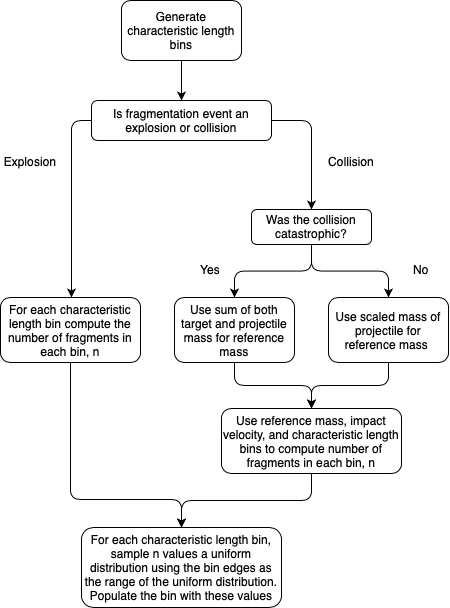
\includegraphics[scale=0.5, trim=0cm 0cm 0cm 5cm]{L_c_flow}
	\caption{The algorithm used for producing the characteristic length distribution used in the NASA breakup model}
\end{figure}

The creation of the characteristic lengths was not given in the original specification of the NASA breakup model by Johnson \citep{johnson_nasas_2001} but was included in the corrections by Krisko in 2001. Krisko specifies that the NASA breakup model deposits fragments of $L_c$ from 1mm to over 1m in bins and that the number of fragments in each bin is determined by a power law that will be discussed later. However, Latizia's implementation for CiELO modified this to first create 100 bins that are equally spaced on a logarithmic scale between 1mm and 10 cm. In this paper, we will be following Latizia's methodology as it has the most up-to-date information about the NASA breakup model. A common theme among the prior research on the NASA breakup model is that each implementation is slightly different due to the lack of information publicly available about the original implementation specified by Johnson et al. \cite{johnson_nasas_2001}. The pieces of debris that are larger than 10cm will be handled separately to ensure that the breakup model conserves mass. Figure ~\ref{bins_sketch} below illustrates the process of using bins to determine the number of fragments of each size.

\begin{figure}[H]
	\centering
	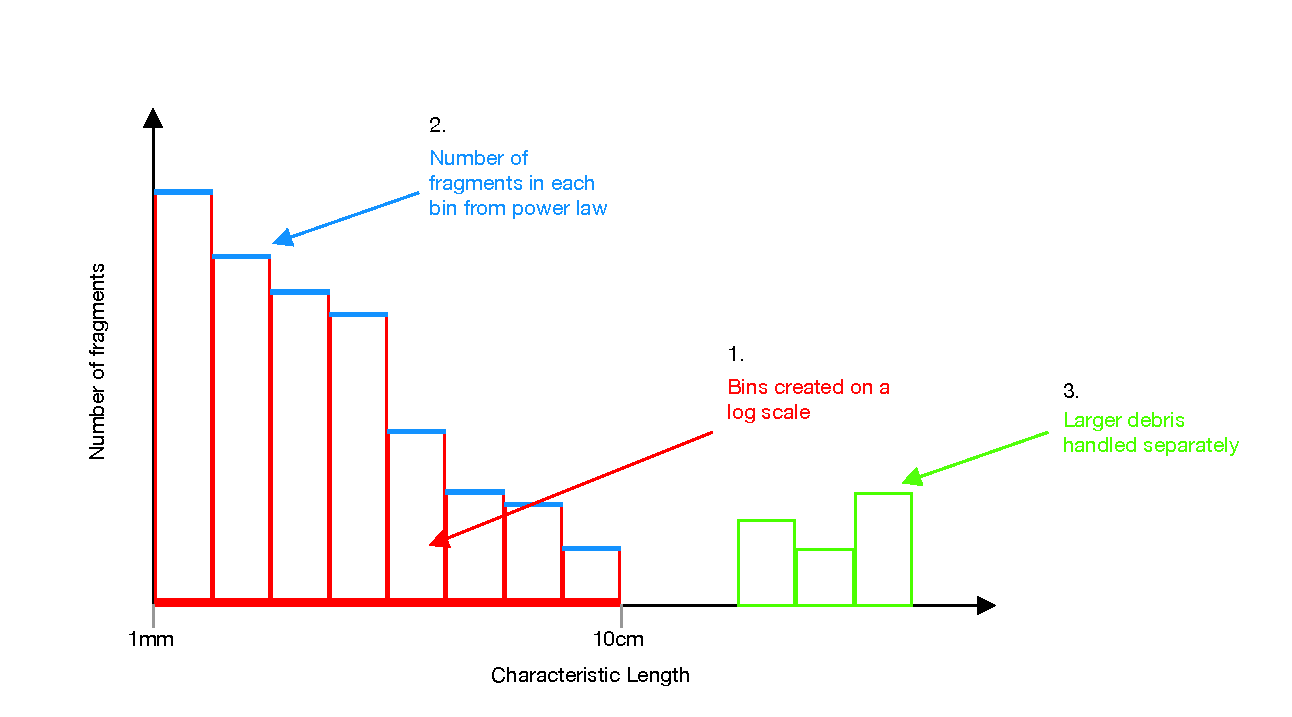
\includegraphics[scale=0.6]{char_len_diagram}
	\caption{A sketch illustrating the process for determining the number of fragments in each characteristic length bin}
	\label{bins_sketch}
\end{figure}

To determine the number of fragments in each characteristic length bin, we acknowledge that collisions and explosions will produce different types of fragments. Explosions will produce larger debris fragments with smaller velocities while collisions tend to generate a large number of small fragments with high velocities \citep{barrows_evolution_1996}.  As such, the number of fragments in each bin will be determined by different power laws based on the type of breakup event.
 
The number of explosive fragments of size \Gls{L_c} is governed by the following equation
\begin{equation}
	N(L_c) =6 S L_c^{-1.6}
\end{equation}
With S = 1, the relationship has been observed to be valid for rocket upper stages with masses in the range of 600-1000 kg \citep{johnson_nasas_2001}. However, for explosions due to other malfunctions such as battery explosions and anti-satellite tests, a value of S between 0.1 and 1 was found to fit the experimental data better \citep{krisko_proper_2011}.

In the case of a collision, a distinction must be made between catastrophic or non catastrophic. A collision is categorized as catastrophic if it causes the complete fragmentation of both the impactor and the target \citep{letizia_space_2016}. This occurs when the energy per target mass exceeds $40 J g^{-1}$ \citep{krisko_proper_2011}. The number of produced fragments for a collision is governed by
\begin{equation}
	N(L_c [m]) = 0.1 (M_e)^{0.75} L_c^{-1.71},
\end{equation}
where \Gls{reference_mass} is defined as follows: 
\begin{equation}
	M_e[kg] = \begin{cases}
		M_t [kg] + M_p[kg]& \text{Catastrophic collision: } \\
		 M_p[kg] * (v_c [km/s] / 1 [km/s])^2 & \text{Non Catastrophic collision}.	
	\end{cases}
	\label{eqn:mass}
\end{equation}
\noindent In equation~\ref{eqn:mass},  \Gls{target_mass} is the target mass, \Gls{prjectile_mass} is the projectile mass, and \Gls{impact_vel} is the relative impact velocity between the target and the projectile.

Figure~\ref{fig:N_f_v_L_c} shows sample results from ODAP to illustrate the characteristic length distribution described above. Additionally, the relevant ODAP function can be found in the appendix in section (X).
\begin{figure}[H]
	\centering
	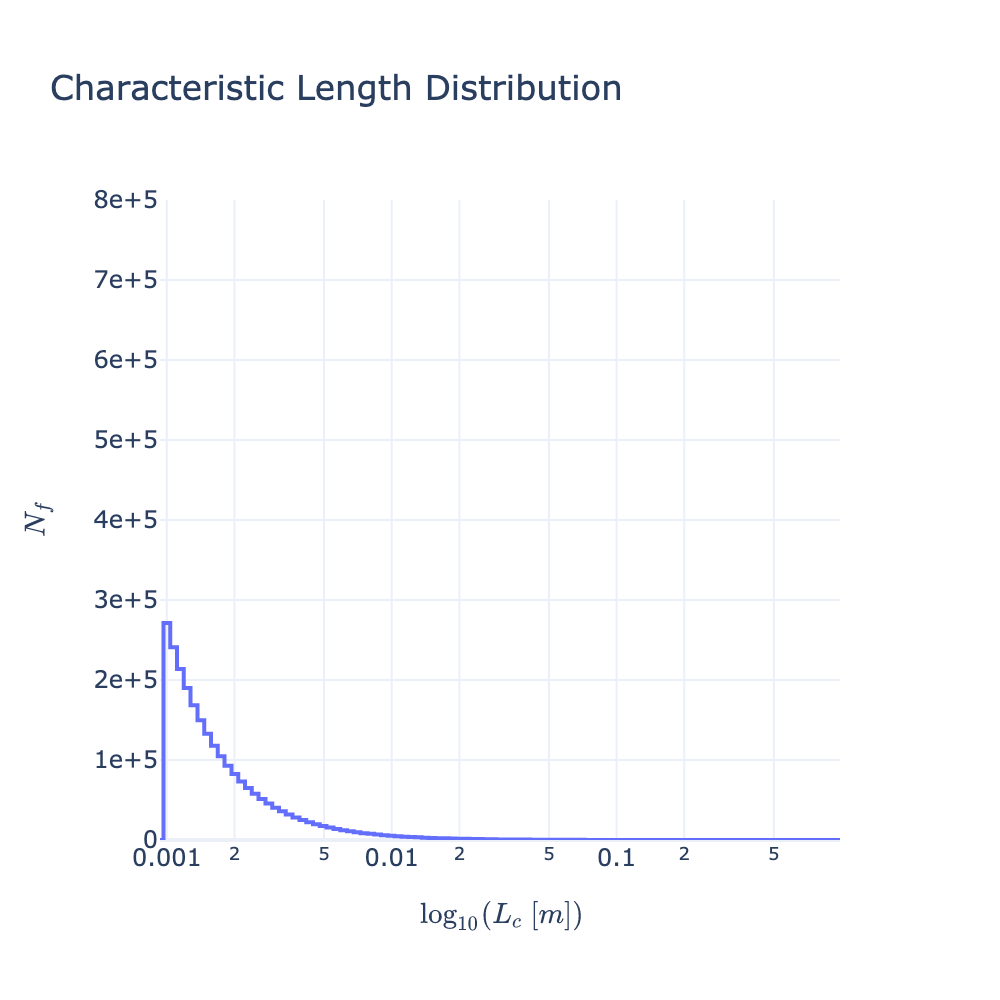
\includegraphics[scale=0.3, trim=0cm 0cm 0cm 10cm]{N_f_vs_L_c}
	\caption{The characteristic length distribution produced by the python implementation of a catastrophic collision involving a rocket body with a mass of 1000kg, a projectile of mass 10kg, and an impact velocity of 10 km/s.}
	\label{fig:N_f_v_L_c}
\end{figure}

\subsubsection{Area to Mass Distribution }

The area-to-mass ratio, $A/M$, for fragments is a distribution that was based on analysis of thousands of fragmentation debris and provides us with a method to determine the mass of each fragment of debris. The discrete distributions were found by using a $\chi^2$ fit to orbital decay characteristics for 1,780 upper stage explosion fragments, and similar data was developed for spacecraft fragments \citep{johnson_nasas_2001}. Each type of debris producer ---RB, SC, and SAT--- will produce different size debris. As such, the distribution that determines the area to mass ratio has three variants. All three are based on a normal distribution but use different expressions for determining the mean and standard deviation of the distribution. For simplicity, the rest of this section will only provide the details of the SC distribution. However, the implementation of the other two categories is included in ODAP.

For small objects with $L_c < 8$cm, SAT, the $A/M$ distribution is expressed as
\begin{equation}
	D_{A/M}(\lambda_c, \chi) = \mathcal{N}(\mu_{A/M}(\lambda_c), \sigma_{A/M}(\lambda_c), \chi).
\end{equation}
$D_{A/M}$ is the distribution function of $\chi$ as a function of $\lambda_c$, where
\begin{align}
	\lambda_c &= \log_{10}(L_c),\\
	\chi &= \log_{10}(A/M)
\end{align}
\Gls{normal_distribution} is the normal distribution function with mean $\mu_{A/M}$ and standard deviation $\sigma_{A/M}$, where
\begin{align}
	 \mu_{A/M} &= \begin{cases} 
		-0.3, & \lambda_c\leq -1.75 \\
		-0.3 - 1.4(\lambda_c + 1.75), & -1.75 < \lambda_c <-1.25 \\
		-1.0, & \lambda_c \geq -1.25 
	\end{cases}\\
	\text{and}\\
	\sigma_{A/M} &= \begin{cases} 
		0.2, & \lambda_c \leq -3.5 \\
		0.2 + 0.1333(\lambda_c + 3.5) & \lambda_c > -3.5 \\
	\end{cases}
\end{align}

Every fragment of debris has a corresponding $A/M$ distribution since both $\mu_{A/M}$ and $\sigma_{A/M}$ are functions of $\lambda_c$. To determine the corresponding $A/M$ ratio for each debris, a random value is drawn from the distribution. This accounts for stochastic nature of breakup events mentioned previously. 

The $A/M$ ratio alone does not provide enough information to determine both the area and mass of a fragment. As such, the average cross-sectional area, $A$, can also be obtained through a one-to-one correspondence with \Gls{L_c} using the following expression \citep{johnson_nasas_2001}:
\begin{align}
	A_x = \begin{cases}
		0.540424 * L_c^2 & \text{where } L_c < 0.00167 \text{ m} \\
		0.556945 * L_c^{2.0047077} & \text{where } L_c \geq 0.00167 \text{ m} \\
	\end{cases}
\end{align}

Utilizing both the $A/M$ ratio and the cross sectional area $A$, we can now obtain the mass $M$ easily using
$M = A_x / (A/M)$.
Figure (X)  shows a simulated A/M distribution and average cross sectional area. The code to reproduce this is found in section (X).
\begin{figure}[H]
	\begin{adjustbox}{max width=1\linewidth,center}
		\centering     %%% not \center
		\subfigure[]{\label{fig:a}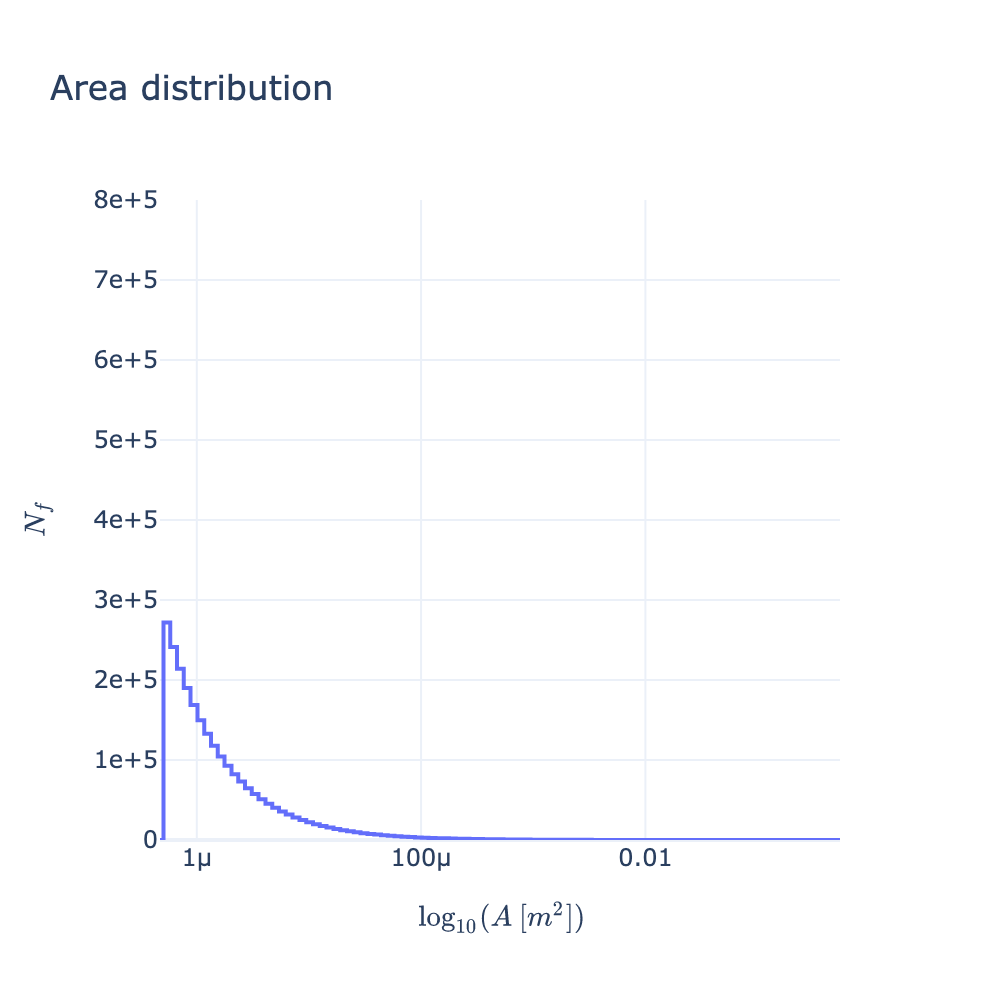
\includegraphics[width=0.5\textwidth]{N_f_vs_A}}
		\subfigure[]{\label{fig:b}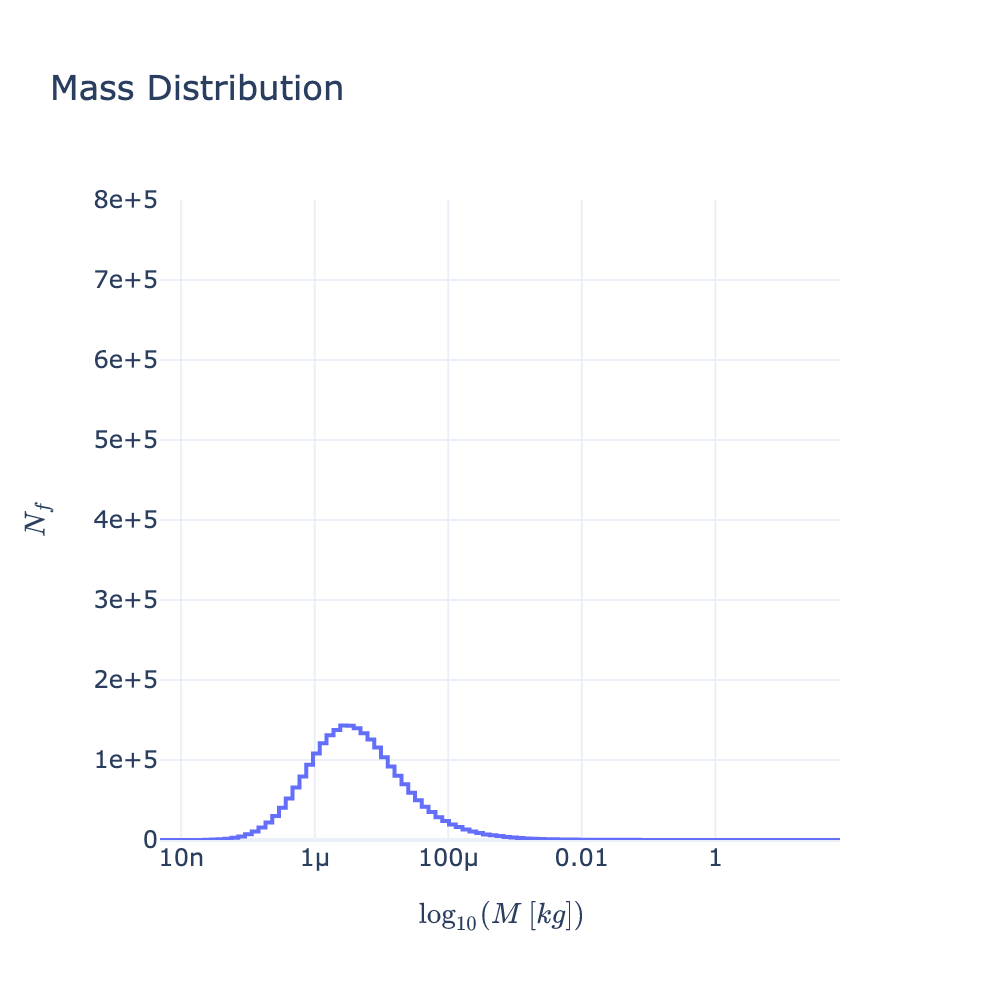
\includegraphics[width=0.5\textwidth]{N_f_vs_M}}
	\end{adjustbox}
	\caption{The characteristic length distribution produced by the python implementation of a catastrophic collision involving a rocket body with a mass of 1000kg, a projectile of mass 10kg, and an impact velocity of 10 km/s. }
\end{figure}

\subsubsection{Change in Velocity Distribution }
The differential amount of velocity that each fragment will gain due to the breakup event is determined in a similar manner to the $A/M$ ratio. The notable differences are that the distribution is now a log-normal distribution and that an additional check is implemented to ensure that extremely high ejection velocities are not included in the case of collisions \citep{letizia_space_2016}. 

More explicitly, the velocity check is performed by sampling a value from the velocity distribution and checking if it is lower than $1.3v_c$, where $v_c$ is the relative collision velocity. If the value fails the check then new values are drawn until the check is passed \citep{letizia_space_2016}.

The change in velocity, \Gls{rel_velocity}, is modeled by log-normal distribution that is function of the $A/M$ ratio by
\begin{equation}
	D_{\Delta v}= \mathcal{N}(\mu_{v}(\chi), \sigma_{v}(\chi), \xi)
\end{equation}
\noindent where \begin{align}
	\xi &= \log_{10}(\Delta v),\\
	\chi &= \log_{10}(A/M),\\
	\mu_{v}(\chi) &= 0.2\chi+1.85,\\
	 \sigma_{v}(\chi) &= 0.4,
\end{align}

The differential velocity vector is constructed by sampling from a uniform distribution for a velocity unit vector and then scaling it with the values from the log-normal distribution. 

It should be noted that details for efficiently handling the resampling of velocities are sparse. As such, ODAP's implementation of the velocity distribution often takes tens of thousands of iterations to complete. One or two fragments often have an area-to-mass ratio that causes the log-normal distribution to be highly unlikely to return a value that is lower than 1.3\Gls{impact_vel}. As such, an iteration limit exists in the code that is set at 100,000 iterations to try and alleviate the computation time. If no suitable value is found before the maximum iteration limit is hit, a value of 1.3\Gls{impact_vel} is assigned to that piece of debris.

\subsection{Validating the Implementation}
Due to the niche nature of orbital debris analysis, it can generally be challenging to find any full implementation of the breakup model. Additionally, many of various space agencies around the world do not share the details of how they implemented the models. For this reason, the above implementations were largely modeled after the details given in the CiELO \cite{letizia_space_2016} which mimicks the information provided in NASA literature.

To validate that ODAP's implementation of the breakup model was performed correctly, a comparison is made to existing data provided by various space agencies for a given scenario. The two scenarios are an explosion event with a rocket body that weighs 1000kg and a catastrophic collision event for a rocket body that weighs 1000kg with a projectile mass that weighs 10kg that has an impact velocity of 10km/s. The data was provided in a presentation given by Rossi et al. \citep{rossi_nasa_nodate}.

As shown in the table~\ref{tab:debris-comparison}, the data from the various space agencies has some significant differences, especially for the characteristic length in the $>$ 1mm range, despite implementing the same NASA breakup model. This is most likely a result of ambiguities in the original NASA breakup model specification literature, as well as differences in how various programming languages perform random sampling. The goal of ODAP is to be within the original deviations of the data.

 
\begin{table}[H]
		\noindent\makebox[\textwidth]{
				\begin{tabular}{|lccccccc|}
				\hline
				\multicolumn{1}{|c|}{\multirow{3}{*}{\textbf{Model}}} & \multicolumn{7}{c|}{Number of Fragments}                                                        \\ \cline{2-8} 
				\multicolumn{1}{|c|}{}                                & \multicolumn{4}{c|}{Length}  & \multicolumn{1}{c|}{Mass} & \multicolumn{1}{c|}{Area} & Velocity \\
				\multicolumn{1}{|c|}{} &
				\textgreater 1mm &
				\textgreater 1cm &
				\textgreater 10cm &
				\multicolumn{1}{c|}{\textgreater 1m} &
				\multicolumn{1}{c|}{\textgreater 1g} &
				\multicolumn{1}{c|}{\textgreater 1cm\textasciicircum{}2} &
				\textgreater 100ms\textasciicircum{}-1 \\ \hline
				ASI                                                   & 378,581   & 9,403  & 234 & 7 & 2,472                     & 5,878                     & 112,932  \\
				CNSA                                                  & 37,865    & 960    & 32  & 9 & 254                       & -                         & 11,380   \\
				DLR                                                   & 1,217,054 & 11,724 & 230 & 0 & 25,844                    & 31,124                    & 31,124   \\
				ESA                                                   & 324,886   & 8,159  & 206 & 6 & 2,093                     & 5,024                     & 98,717   \\
				NASA                                                  & 434,928   & 10,731 & 248 & 8 & 2,525                     & 6,416                     & 132,032  \\
				\textbf{\textit{ODAP}}                        & 378,525         & 9,479     & 223  & 6 & 3613                         & 5,850                         & 120,481        
		
				\\ \hline
			\end{tabular}
		}
		\caption{(Data Source: NASA Breakup Model Implementation Comparison of results, A. Rossi, 24th IADC Meeting April 2006) }
		\label{tab:debris-comparison}
\end{table}


\newpage
\section{State Representation}

Following the successful computation of the fragmentation event, we need to construct a state representation for each piece of orbital debris. There are two primary methods for representing the state of an orbital body.

The first is using \boldindex{orbital state vectors} to represent the debris. Orbital state vectors consist of the Cartesian position, $\vec{r}$, and velocity $\vec{v}$ along with time, $t$. Additionally, the preferred coordinate system for this representation is the \boldindex{Earth-Centered Inertial (ECI) Coordinate system}. This is a coordinate frame with the origin at the center of Earth's mass and has orbiting satellites moving relative to Earth. The orbital state vector representation is a natural result of Newton's laws of motion and the universal law of gravitation.

The second representation is using \boldindex{Keplerian elements}, which result from Kepler's laws of planetary motion. These consist of the eccentricity, \emph{e}, Semimajor axis, \emph{a}, inclination, \emph{i}, longitude of the ascending node, $\Omega$, the argument of periapsis, $\omega$, and the true anomaly, $\nu$. 

Both of these methods have advantages and disadvantages for modeling orbital debris, and as such, it is often convenient to switch back and forth between them. Keplerian elements are a more abstract representation of an object's motion but provide significant benefits for performing propagations forward in time. Orbital state vectors are often more suited to performing visualizations and give a more intuitive sense of each piece of debris's current state. Both of these representations are explored in this section, as well as their benefits and construction.

\subsection{Orbital State vectors and their advantages}

The orbital state vectors utilize Newton's laws of motion and Newton's universal law of gravitation to describe the motion of an object in space. 
Newton's universal law of gravitation states that $$\vec{F}_{grav} = G\frac{ m_1 m_2 \vec{r}}{\mid\vec{r}\mid^3}$$ \noindent This is the dominant force that acts on orbital objects, neglecting drag. As such, application of Newton's second law yields
\begin{align}
	m_1 \vec{a_1}  & = G\frac{m_1 m_2 \vec{r}}{\mid\vec{r}\mid^3}\\
	\vec{a_i}  &= G \sum_{i \ne j}  m_j \frac{\vec{r_j} -\vec{r_i}}{\mid\vec{r_j} - \vec{r_i}\mid^3} \indent\text{(More general)}
\end{align}

Therefore, the change in an object's velocity can be expressed as the sum of the contributions of gravitational attraction from all other surrounding bodies. Gravitational force depends on mass, meaning the gravitational attraction for a piece of debris to nearby debris is negligible compared to the gravitational attraction from a nearby planetary body. Thus, for computational efficiency, inter-particle interactions will be neglected.

The benefits of using orbital state vectors are that they provide a natural intuition for how the motion of a piece of debris will change over time and they provide the necessary information for 3D visualization. However, a large drawback of using state vectors is that all six degrees of freedom, $ (x, y, z, v_x, v_y, v_z)$, will be changing during each timestep. As such, when simulating a large number of fragments orbiting a body, the memory usage will grow quite large. Additionally, the periodic nature of orbits is not captured with this parameterization. More precisely, knowing the state of a piece of debris in the far future will require propagating that debris from its initial conditions up to the desired time step. This is an undesirable consequence and one of the primary motivations for preferring the Keplerian element parameterization.
 
\newpage
\subsection{Keplerian elements and their advantages}

When viewed from an inertial plane, two orbiting bodies trace distinctive trajectories, where each has a focus at the common center of mass.  When switching to a non-inertial frame centered on one of the bodies, only the opposite body's trajectory is viewable. Keplerian elements are a parameterization that describes these non-inertial trajectories (Wikibook). *** FIX

The reference body is called the primary body. In our case, this is the Earth, while the other body is called the secondary body. It should be noted that there is no preferred primary or secondary body.

The first step to reparameterize the motion of the orbital debris is to use the position vector, $\vec{r}$, and velocity vector, $\vec{v}$, to define the \boldindex{specific angular momentum} vector as
\begin{equation}
\vec{h} = \vec{r} \times \vec{v}.
\end{equation}
Using the Earth's equator as the \boldindex{fundamental plane}, which is the plane that is used as a reference, we can begin constructing the parameters of the \boldindex{orbital plane}---the plane created by tracing out the $\vec{r}$ vector, which contains both the $\vec{r}$ and $\vec{v}$. The intersection of the orbital plane with the fundamental plane is called the \boldindex{line of nodes}.

The \boldindex{ascending node} is the spot where the orbiting body crosses the plane of reference/equatorial plane in a northerly direction. Similarly, the \boldindex{descending node} is where it crosses the plane of reference in a southerly direction. The vector $\vec{n}$ points in the direction of the ascending node and is found by taking the cross product of the unit vector $\hat{k}$ with the angular momentum $\vec{h}$.
\begin{equation}
\vec{n} = \hat{k} \times \vec{h}
\end{equation}

\begin{figure}[t]
	\centering
	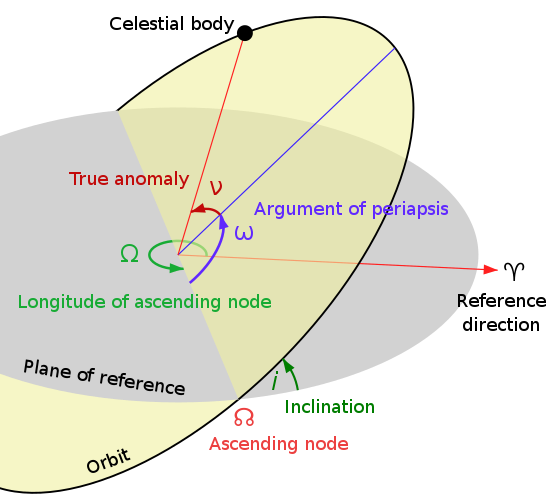
\includegraphics[scale=0.35]{keplerian-elements}
	\caption{A diagram illustrating the Keplerian elements related to the orbital plane intersecting a reference plane. Data Source: Orbital elements Wikipedia page }
\end{figure}

The \boldindex{semi-major axis}, $a$,  is one half of the major axis. The major axis is a line that goes through both foci of the ellipse and the center and ends at the widest point of the perimeter.

\begin{figure}[h]
	\centering
	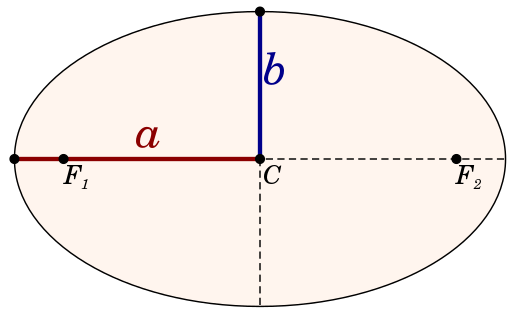
\includegraphics[scale=0.35]{semi-major_and_minor_axes}
	\caption{The semi-major axis, a, along with the semi-minor axis, b, and the foci of an ellipse, $F_1$ and $F_2$. Data Source: Semi-major and semi-minor axis Wikipedia page}
\end{figure}

Using the vis-viva equation, the semi-major axis, $a$, can be defined as
\begin{equation}
a = \frac{1}{\frac{2}{\mid \vec{r} \mid} - \frac{\mid \vec{v} \mid^2 }{\mu}},
\end{equation}
\noindent where $\mu$ is the standard gravitational parameter of the primary body. For Earth, the value of $\mu$ is $3.986 *10^{14}\text{m}^3/\text{s}^2$.

The \boldindex{orbital eccentricity} is a dimensionless parameter that indicates to what degree an orbit around another body deviates from a perfect circle. It has the value of 0 for a circular orbit, a value between 0 and 1 for elliptic orbits, 1 for parabolic escape orbits, and greater than 1 for hyperbolic orbits. For the purpose of orbital debris in LEO, the eccentricities will be in the elliptic orbit range.

The equation for eccentricity can be expressed from the the orbital state vectors as follows:
\begin{equation}
\vec{e} = \left(\frac{\mid \vec{v} \mid^2}{\mu} - \frac{1}{\mid \vec{r} \mid}\right)\vec{r} - \frac{(\vec{r} \cdot \vec{v})}{\mu}\vec{v}
\end{equation}

\begin{figure}[h]
	\centering
	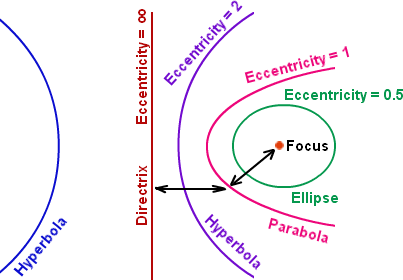
\includegraphics[scale=0.45]{eccentricity}
	\caption{The relationship between the eccentricity and the resulting conic section. Data Source: https://3.bp.blogspot.com}
\end{figure}

The \boldindex{inclination}, \textit{i}, is the angle formed between the unit vector pointing in the $\hat{k}$ direction and can be calculated by
\begin{equation}
\textit{i} =  \arccos \frac{K_z}{\mid \vec{h} \mid},
\end{equation}
where $\vec{h}$ is the angular momentum.

The \boldindex{true anomaly}, $\nu$, is used to define the position of the body in its orbit, and is the angle between the direction of the periapsis and the current position of the body.
\begin{equation}
	\nu [rad] = \begin{cases}
		\arccos \frac{\vec{e} \cdot \vec{r}}{\mid \vec{e} \mid \mid \vec{r} \mid} & \text{for } \vec{r} \cdot \vec{v} \geq 0 \\
		2\pi - \arccos \frac{\vec{e} \cdot \vec{r}}{\mid \vec{e} \mid \mid \vec{r} \mid}& \text{otherwise}	
	\end{cases}
\end{equation}


 The \boldindex{eccentric anomaly}, $E$, is also used to measure an object's position in an orbit. The eccentric anomaly is defined using the magnitude of the eccentricity vector, $e = \mid\vec{e}\mid$, and  the true anomaly as follows:

\begin{equation}
	E = 2\arctan \frac{\tan \frac{\nu}{2}}{\sqrt{\frac{1 + e}{1-e}}}
\end{equation}

The \boldindex{longitude of the ascending node}, $\Omega$, is the angle between the ascending node and the unit vector $\hat{i}$
\begin{equation}
	\Omega [rad] = \begin{cases}
		\arccos \frac{n_x}{\mid \vec{n} \mid} & \text{for } n_y \geq 0 \\
		2\pi -	\arccos \frac{n_x}{\mid \vec{n} \mid} & \text{for } n_y < 0.
	\end{cases}
\end{equation}

The \boldindex{argument of periapsis}, $\omega$, is the angle in the orbital plane that is between the ascending node and the periapsis and is calculated using
\begin{equation}
	\omega [rad] = \begin{cases}
		\arccos \frac{\vec{n} \cdot \vec{e}}{\mid \vec{n} \mid \mid \vec{e} \mid} & \text{for } e_z \geq 0 \\
		2\pi -\arccos \frac{\vec{n} \cdot \vec{e}}{\mid \vec{n} \mid \mid \vec{e} \mid}& \text{for } e_z < 0	
	\end{cases}
\end{equation}

Finally, using \boldindex{Keplers equation} we can define the \boldindex{mean anomaly} as
\begin{equation}
	M = E - e\sin E
\end{equation}

We can now parameterize each of the debris fragments using ($e$, $a$, $i$, $\Omega$, $\omega$, $M$). This step is crucial to ensure that in the absence of orbital perturbations, only one of these parameters, the mean anomaly, will change with respect to time, $t$. This will allow for more efficient computations in the band formation phase of the simulation. Moreover, the change in mean anomaly with respect to time is analytic and expressed as
\begin{equation}
\frac{dM}{dt} = \sqrt{\frac{\mu}{a^3}}.
\end{equation}

As such, the position of a piece of debris in orbit can be found at any time in the future without having to numerically approximate its change in position over time. Due to the vast amount of debris generated, this will provide major benefits for the band formation phase of the orbital debris cloud.

\newpage
\section{Debris Cloud Evolution}

Debris cloud evolution is the collective change in the orbits and positions of fragments with respect to time. This evolution goes through a few distinctive phases, notably the ellipsoid,  ring formation, toroid, and band formation, as illustrated in Figure~\ref{fig:debrisphases}. In addition to having different shapes, those phases differ in how long they last and the type of model used to describe them. For example, the ellipsoid and ring formations occur within a few days. As such, only the force of gravity  will have a significant effect during this period.  However, the toroid and band formation phases take over a year. As a result, additional forces such as drag will have more prominent effects due to the increased duration. Different methodologies need to be applied for each phase to ensure fast and accurate computations. These different phases, the forces being considered, and the methodologies used will be analyzed in-depth in the following subsections.
\vspace{\baselineskip}

\begin{figure}[h]
	\centering
	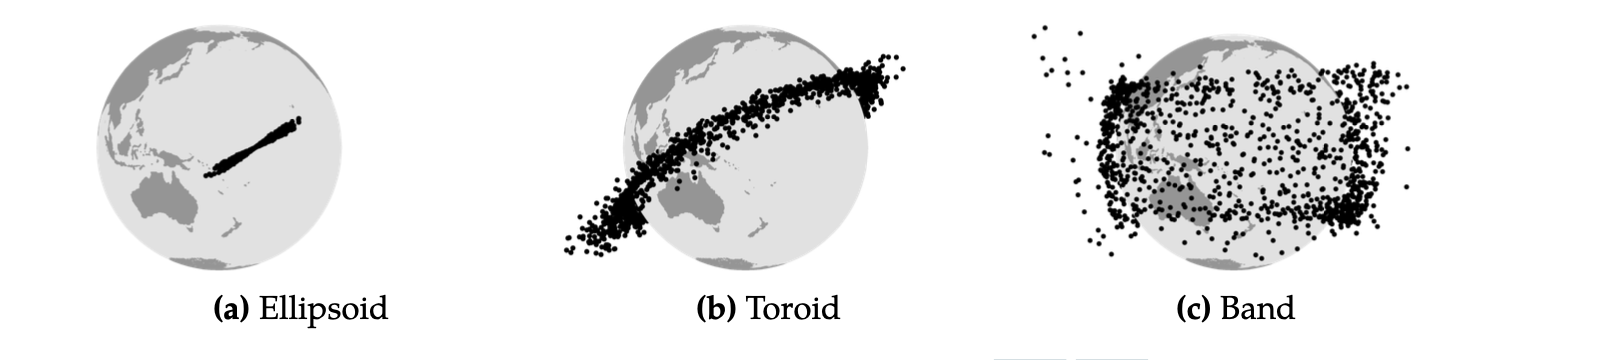
\includegraphics[scale=0.45]{debrisphases}
	\caption{The three phases of debris cloud evolution. Data Source: Letizia}
	\label{fig:debrisphases}
\end{figure}


\subsection{Ellipsoid and Ring Phase}

At the time of the fragmentation event, all debris fragments have the same position. However, as seen in Section 2, each fragment has a different velocity in both direction and magnitude. This causes the debris to spread out and form first and ellipsoid (Figure ~\ref{fig:ellipsoid}) then a complete ring around the Earth. As the debris cloud expands, the number of other satellites it can potentially impact grows. On the other hand, the cloud also gets sparser, and the probability of any specific satellite getting hit decreases. In other words, the odds of subsequent collision spread out as well.

\begin{figure}[h]
	\centering
	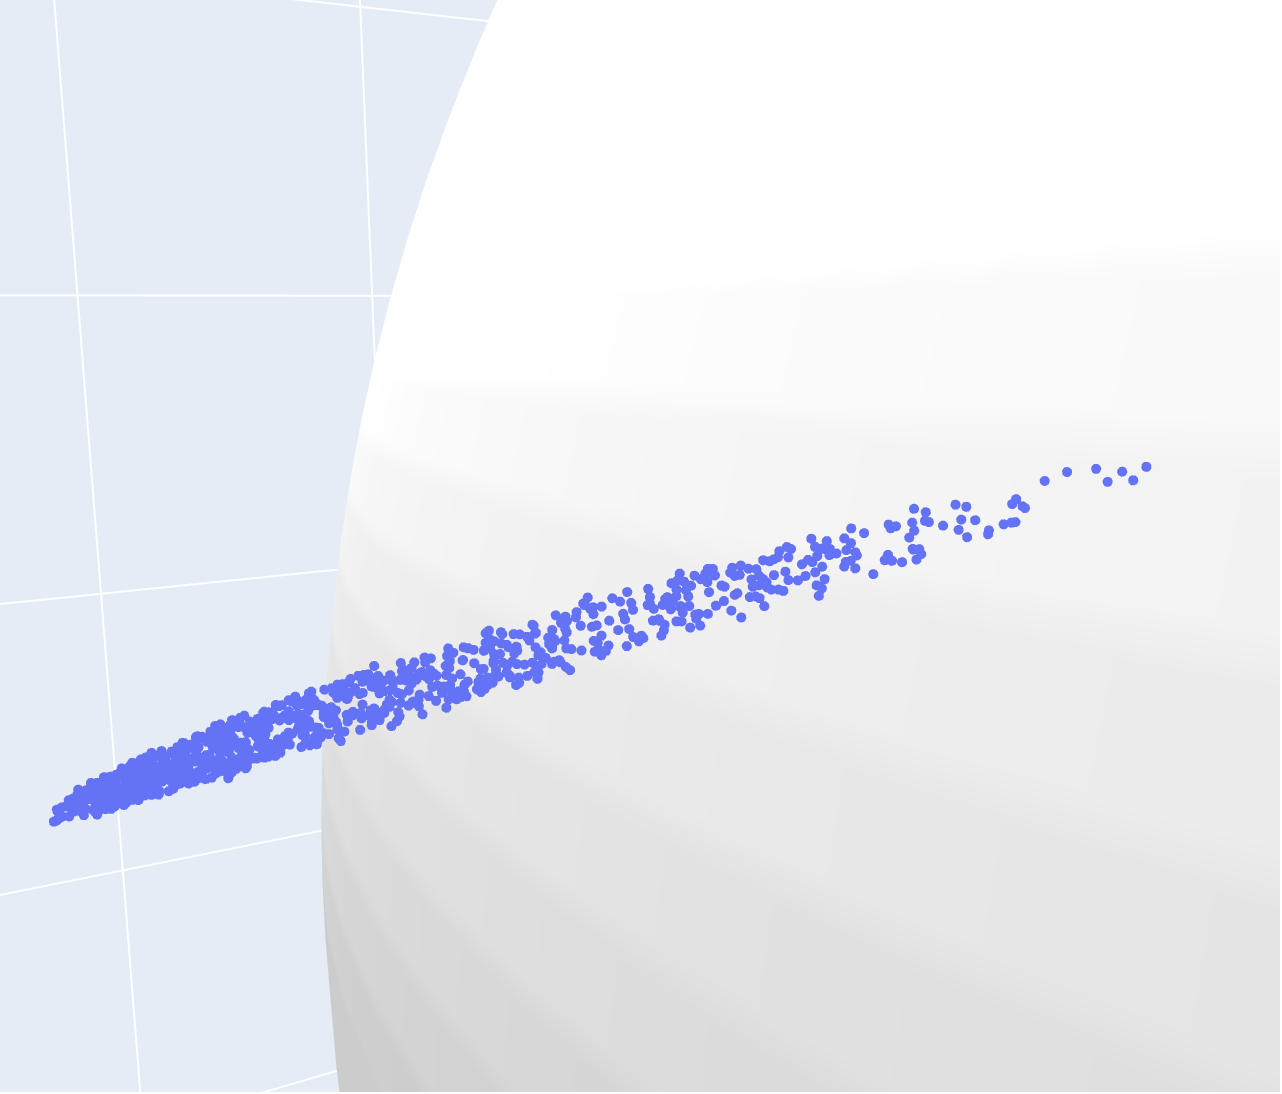
\includegraphics[scale=0.35]{ellisoid_phase}
	\caption{A visualization created by ODAP of the ellipsoid formation occurring.}
	\label{fig:ellipsoid}
\end{figure}

It takes two to three days for the debris to form a uniform ring around the Earth. On this time scale, weak effects such as air drag and gravitational forces between debris are negligible. As a result, each debris fragment orbits around the Earth as if the other fragments did not exist. From a practical point of view, we can use standard results for the two-body gravitational problem (CITE TEXTBOOK).

While the two-body problem is well characterized, it is not computationally efficient enough to perform long duration and accurate propagation. As such, we reframe the problem as propagating Kepler orbits.

\boldindex{Kepler orbits} are orbits in which no perturbations of inter-gravitational interactions are considered---a special case of the two-body problem. Framing the problem this way lends itself naturally to using Keplerian elements. For Kepler orbits, only the orbits' anomalies will be changing over time, which reduces the number of computations that need to be performed and aids in maintaining accuracy.

This benefit is a result of \boldindex{Kepler's Equation}, which is expressed in terms of the mean anomaly as
\begin{equation}
	M = E - e\sin(E) = \sqrt{\frac{\mu}{a^3}}\left(t - t_0\right),
\end{equation}
where $E$ is the eccentric anomaly, $e$ is the eccentricity, $\mu$ is the standrad gravitational parameter, $a$ is the semi-major axis, $t$ is some time in the future, and $t_0$ is the current time. Since we have an analytic expression for the mean anomaly, we do not need to use any integration methods for propagating Kepler orbits forward in time. This results in the aforementioned computational efficiencies.

The next step is to find the corresponding eccentric and true anomalies from the propagated mean anomaly. The eccentric anomaly is found from the Kepler equation; however, there is no closed-form solution given the mean anomaly. As such, numerical integration must be used to find the eccentric anomaly. The processes for performing the integration of Kepler's equation are the subject of many other research papers due to the importance it plays in orbit propagation. It is not included in this paper for conciseness, but a python implementation of one of the methods can be found in the appendix in section (TO DO INSERT REFERENCE TO APPENDIX SECTION HERE)(Maybe talk about the new methods in this area that do not require using integration).

Kepler's equation has another form which enables us to convert the resulting eccentric anomaly to the true anomaly. This form is given as
\begin{equation}
	\nu = 2 \arctan\left(\sqrt{\frac{1+e}{1-e}}\tan\frac{E}{2}\right).
\end{equation}

Since we now have expressions for how the three anomalies will change over time for Kepler orbits, we can accurately propagate the debris until the ring formation phase is completed. However, we now need to have a method to detect once the ring formation phase is completed to switch to performing the propagation for future phases. A visualization of end result of the ring formation phase is provided in Figure~\ref{ring}.
\begin{figure}[b!]
	\centering
	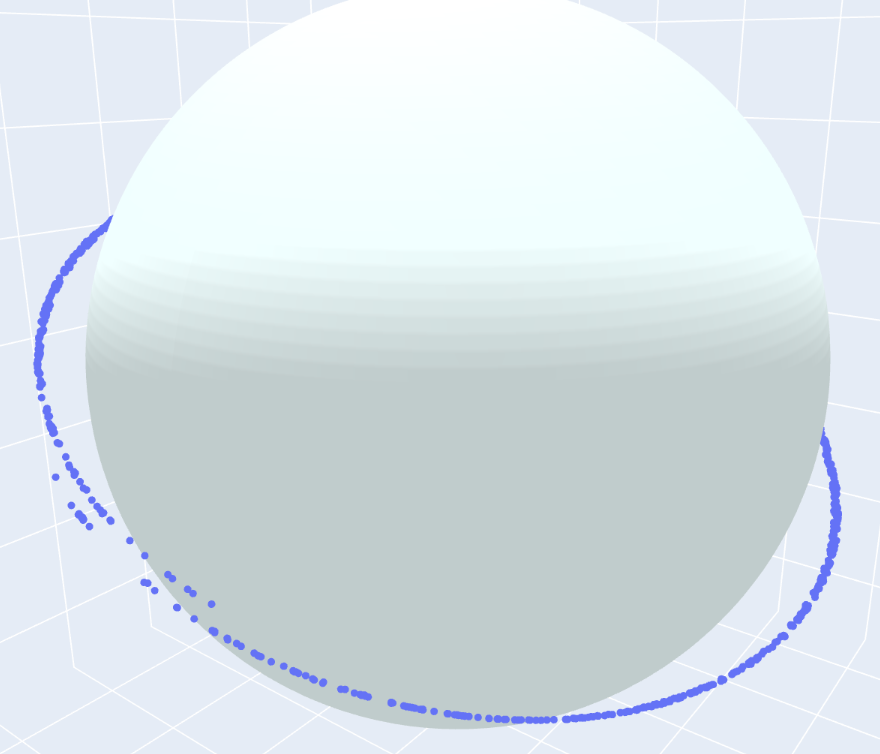
\includegraphics[scale=0.45]{ring_phase}
	\caption{A visualization created by ODAP of the completed ring formation.}
	\label{ring}
\end{figure}

\subsection{Transition to Toroid and Band Phase}

Detecting the end of the ring formation phase is crucial in propagating the debris cloud. When transitioning from the ring phase to the toroid and band phases, additional forces such as drag must be considered. Additionally, these new phases take a much longer amount of time to form. Both of these factors result in needing to switch to a new propagation method. As such, detecting when the ring has formed allows us to switch to this new propagation method.

To asses whether the system has formed a roughly uniform ring, we monitor the amount of debris passing through a certain region of space as a function of time. A visualization of how this process works is provided in Figure~\ref{flux_diagrams}.

\begin{figure}[h]
	\begin{adjustbox}{max width=1\linewidth,center}
		\centering     %%% not \center
		\subfigure[]{\label{fig:a}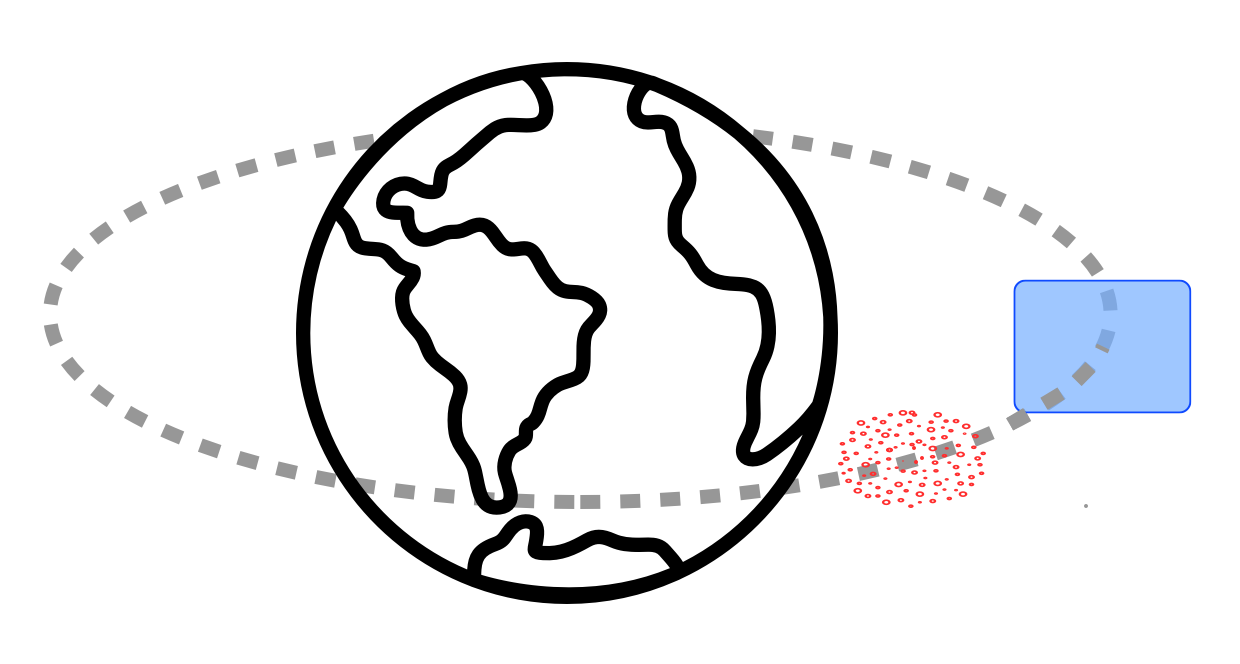
\includegraphics[width=0.5\textwidth]{Flux_diagram1}}
		\subfigure[]{\label{fig:b}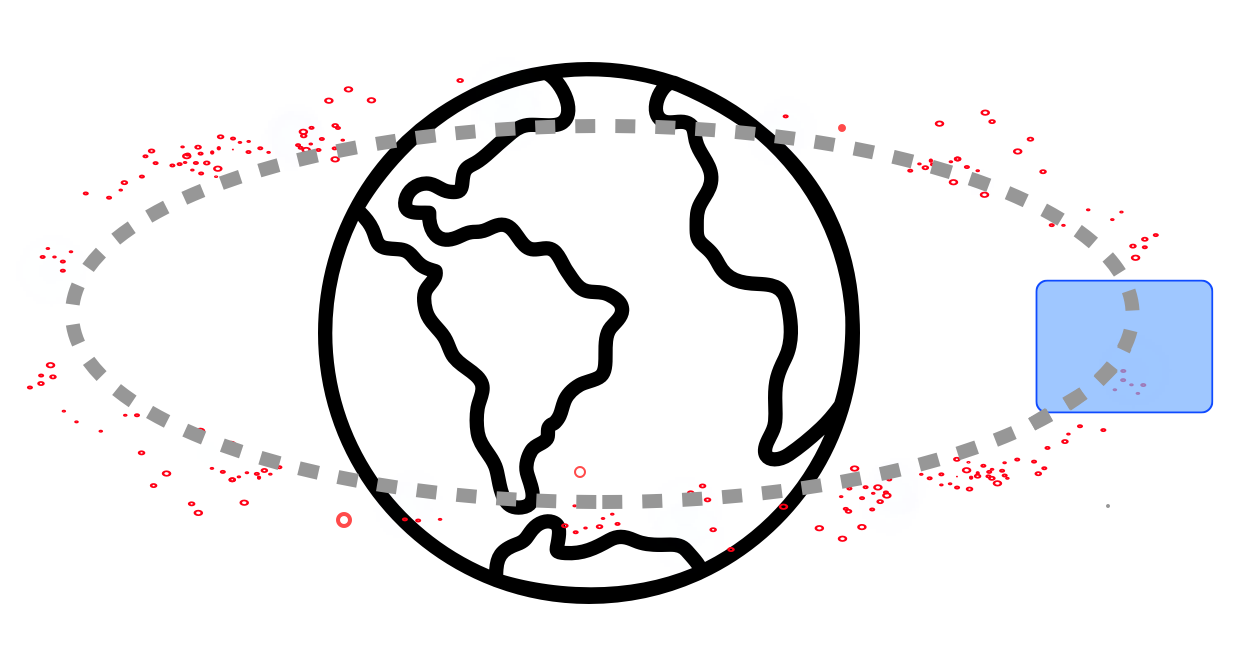
\includegraphics[width=0.5\textwidth]{Flux_diagram2}}
	\end{adjustbox}
	\caption{Measuring the flux at the time of the ellipsoid phase \textbf{(a)} and measuring the flux near the completion of the ring phase \textbf{(b)} }
	\label{flux_diagrams}
\end{figure}

More specifically, to measure the fragments' spread we will define a particle-based flux. This is accomplished by creating an $xz$-plane in the equatorial coordinate system and detecting when particles have switched from one side of the plane to the other. Plotting the results will show peaks when the fragments pass through, which will converge to some value as the fragments become uniformly spread out.

Plotting the flux over time shows these expected peaks and what seems to be convergence to some value. However, the data is quite noisy and we need a concrete method to determine when the fragments will be distributed uniformly. As such, we need to develop a method to test for when the data has converged. A property that is true of all uniform distributions is that the variance approximately equals the mean. As such, we can define a convergence ratio using the variance and mean of the flux. When the convergence ratio is within some defined tolerance we can test for when the flux has become uniform. Once the convergence ratio is within the defied tolerance  we can then conclude that the ring formation phase has completed. It should be noted that the ring never reaches true uniformity which results in oscillating flux. An example of how the flux and convergence ratio evolves with time is shown in Figure~\ref{flux_plots}.

\begin{figure}[t]
	\begin{adjustbox}{max width=1\linewidth,center}
		\centering     %%% not \center
		\subfigure[]{\label{fig:a}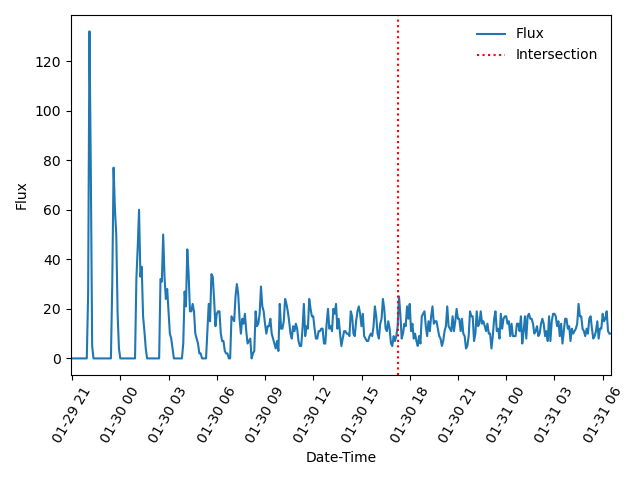
\includegraphics[width=0.5\textwidth]{Flux_v_Time}}
		\subfigure[]{\label{fig:b}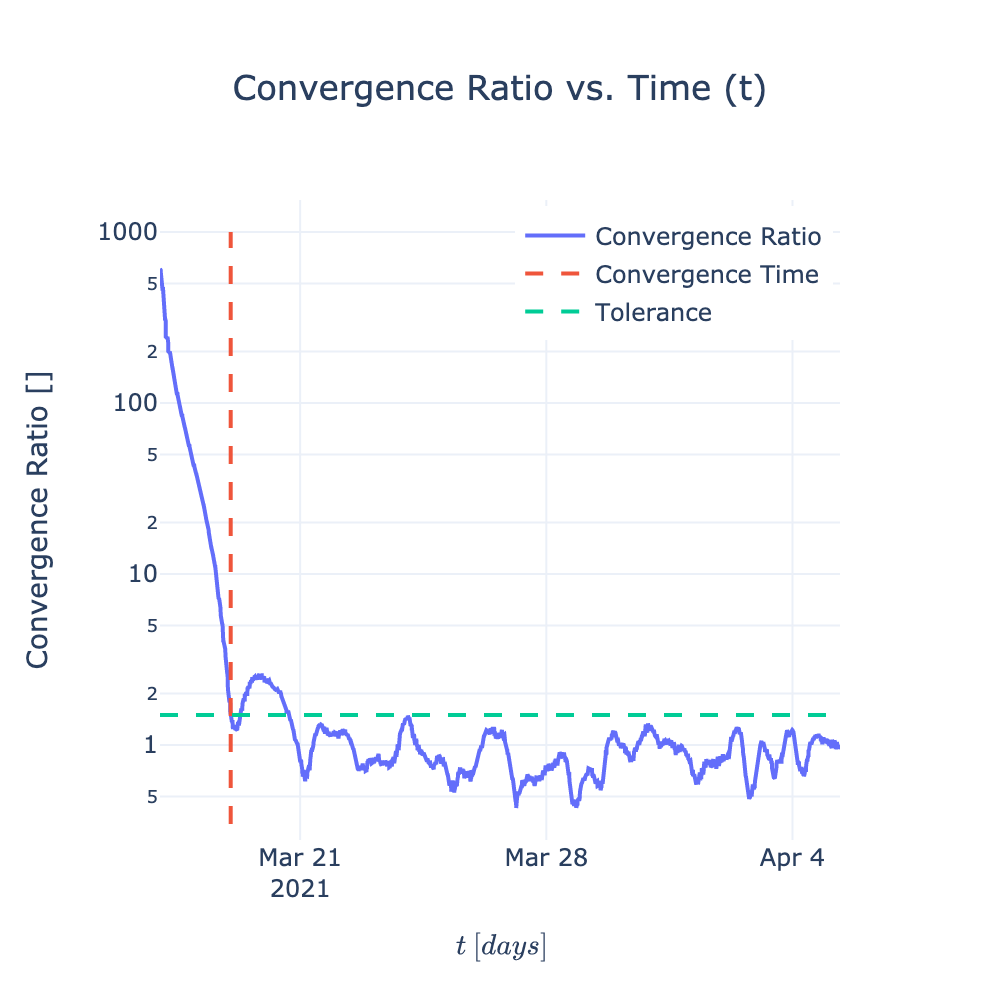
\includegraphics[width=0.5\textwidth]{Convergence_Ratio_v_Time}}
	\end{adjustbox}
	\caption{The flux of the fragments as a function of time \textbf{(a)} and the convergence ratio of the flux as a function of time \textbf{(b)} }
	\label{flux_plots}
\end{figure}


\subsection{Toroid and Band Phase}
For the evolution of the cloud to continue, we must now consider orbital perturbations that will cause the orbits to change over time. Beginning to consider perturbations such as drag and J2 will enable the ring shape of the cloud to evolve towards the Toroid band. 

\subsubsection{Aerodynamic Drag}

A significant perturbation that causes changes in the fragments' orbits is \boldindex{atmospheric drag}. Atmospheric drag acts on a fragment as a result of molecules in the atmosphere colliding with its surface and is a natural consequence of conservation of momentum. 

\subsubsection{Atmospheric Models}

To model the effects of drag, a suitable atmospheric model must be selected. An atmospheric model tells us information about factors such as air pressure, air density,and wind speed at varying locations in the atmosphere. However, it would be cumbersome and computationally inefficient to utilize a model that contains all of this information.  As such, atmospheric models tend to focus on a select few variables rather than creating a universal ``best'' model that considers all relevant factors \citep{vallado_d._2013}.

Choosing a model that best fits a given use case comes down to the desired criterion for speed, accuracy, and applicability. For example, the DAMAGE orbital debris model assumes a rotating, oblate atmosphere with density and density scale height values taken from the 1972 COSPAR International Reference Atmosphere (CIRA) \citep{soton388786}.  A detailed exploration of various atmospheric models is given by Gaposchkin and Coster \citep{Gaposchkin1988AnalysisOS}, but for the purposes of this paper, we will be focusing on a model called the \boldindex{exponential atmospheric model}. This is a  a static model that assumes a spherically symmetric distribution of particles, where the density decays exponentially with increasing altitude \citep{vallado_d._2013}.

In the exponential atmospheric model the air density $\rho$ varies according to
\begin{equation}
	\rho = \rho_0\:\exp\left(-\frac{h_{ellp} - h_0}{H}\right)
\end{equation}
where $\rho_0$ is a reference density that is used with $h_0$,  a reference altitude,  $h_{ellp}$ is the actual altitude above the ellipsoid, and $H$ is a scale height.

The reference density and reference altitude are tabulated values that come from sources such as the U.S. Standard Atmosphere and CIRA. The scale height is a value used to ensure continuity throughout $\rho$. The combination of the U.S. Standard Model and CIRA will yield moderately accurate results for general purposes and as such will utilized in for computing the force of drag \citep{vallado_d._2013}. \footnote{The atmospheric model implementation, including the tabulated values that are used, are included in the appendix of this paper}

\begin{figure}[h]
	\centering     %%% not \center
	%\vspace*{-1.5in}
	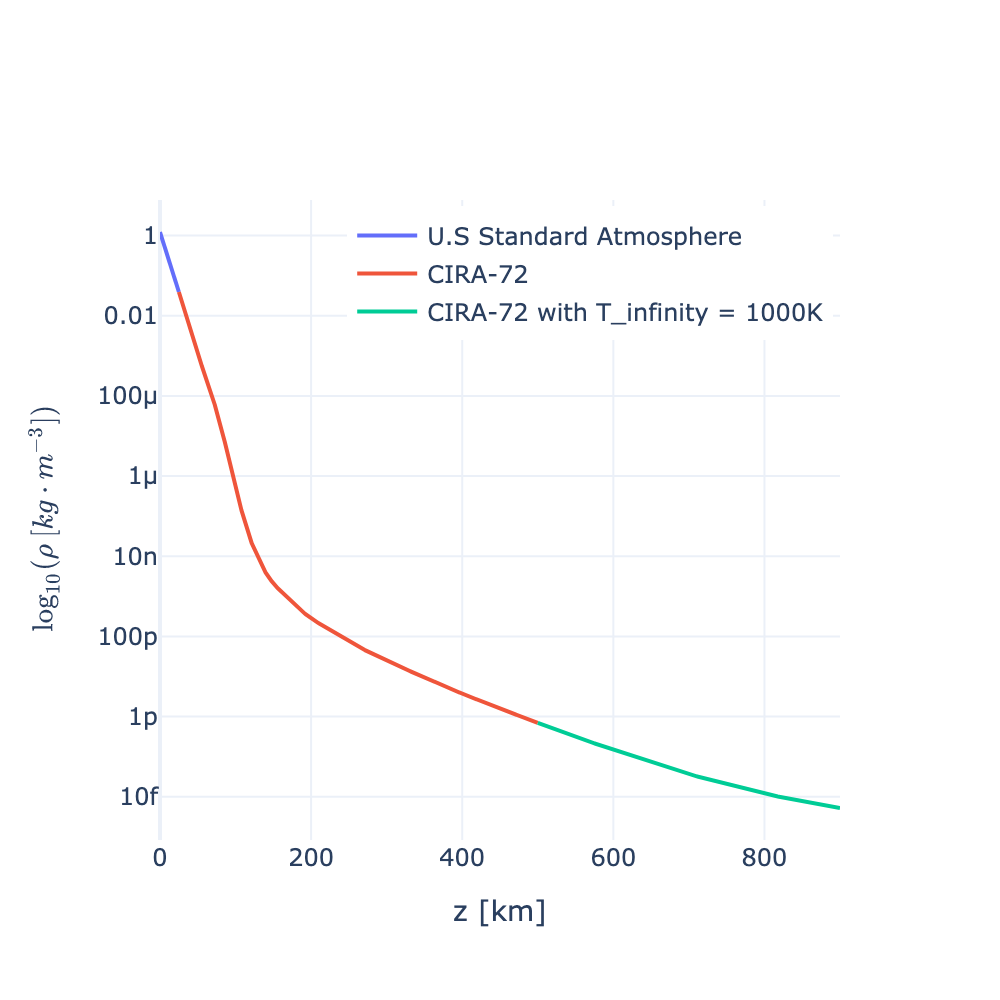
\includegraphics[width=0.7\textwidth]{Atmospheric_Density_v_Altitude}
	\caption{The atmospheric density of Earth as a function of altitude according to the Exponential Atmospheric Model}
\end{figure}

The air density, $\rho$, as a function of altitude is shown above. Note that the $y$-axis is given as a log scale due to the rapidly increasing density of air at high altitudes as the distance to Earth shrinks.

\subsubsection{Effects of Drag on Orbital Elements}

The aerodynamic drag on an object is typically expressed in the following form:
\begin{equation}
	F_D = \frac{1}{2m} \rho v^2 \: C_D A
\end{equation}
where $\rho$ is the air density, $v$ is the speed of the object relative to the fluid, $C_D$ is an experimentally determined dimensionless number, $A$ is the cross sectional area, and $m$ is the mass of the satellite.

Drag is a force that will cause an acceleration that opposes the direction of motion of an object. As such, drag produces a similar effect to a retrograde thrust which enables aerobraking, a useful orbital maneuver that can be performed around planetary bodies with an atmosphere. Similarly, for orbital debris, drag is the predominant force behind changing the semi-major axis and eccentricity, gradually causing the debris to have a lower perigee.

As a result of the density increasing exponentially as altitude decreases, the effects of drag create a form of a feedback loop. A satellite experiences drag, which lowers its orbit, which in turn causes it to experience more drag. This will continue until a satellite is eventually deorbited. 

The expressions for the effects of drag on orbital elements are derived by King-Hele and cover three different ranges of eccentricities \citep{KINGHELE1987269}.

\begin{align}
		\dfrac{da}{dt} = \begin{cases}
			-\dfrac{C_D A}{M} \sqrt{\mathstrut\mu_E a \rho} \exp\left(-\dfrac{a - R_h}{H}\right)[I_0 
			+ 2eI_1 + \\ \:\:\:\dfrac{3}{4}e^2(I_0 + I_2) + \dfrac{e^3}{4}(3I_1 +I_3)] & \text{for } 0.01 \leq e \leq 0.2 \\[2ex]
			-\dfrac{C_D A}{M} \sqrt{\mathstrut\mu_E a \rho}\exp\left(-\dfrac{a - R_h}{H}\right)\left[I_0 + 2eI_1 \right] & \text{for } \text{for } 0.001 \leq e < 0.01\\[2ex]
			-\dfrac{C_D A}{M} \sqrt{\mathstrut\mu_E a \rho}\exp\left(-\dfrac{a - R_h}{H}\right) & \text{for } e < 0.001\\[2ex]
		\end{cases}\\
		\newline
		\dfrac{de}{dt} = \begin{cases}
			-\dfrac{C_D A}{M} \sqrt{\mathstrut\dfrac{\mu_E}{a} \rho}\exp\left(-\dfrac{a - R_h}{H}\right) & \text{for } 0.01 \leq e \leq 0.2  \\[2ex]
			-\dfrac{C_D A}{M} \sqrt{\mathstrut\dfrac{\mu_E}{a} \rho}\exp\left(-\dfrac{a - R_h}{H}\right)\left[I_1 + \dfrac{e}{2}(I_0 + I_2)\right] & \text{for } 0.001 \leq e < 0.01\\[2ex]
			0 & \text{for } e < 0.001\\[2ex]
		\end{cases}
	\end{align}

$I_k(z)$ represents the modified Bessel function with order $n$, where $z = \frac{ae}{H}$ and is given by
$$
I_k(z) = \dfrac{1}{\pi} \int_{0}^{\pi} e^{z\cos(\theta)}\cos(k\theta)d\theta \:\:\:\:\:\: k \in \mathbb{Z}.
$$

Following the precedents of many other texts, we will be assuming that the fragments have a drag coefficient of 0.7. Modifications were made by Frey et al. to find more appropriate boundary conditions and to increase the accuracy of each phase by including more terms of the series expansion \citep{frey_extension_2019}.

The first modification to the King-Hele implementation is to introduce two functions, $k_a$  and $k_e$, that are used for describing the rate of change of $a$ and $e$ in all eccentricity regimes \citep{frey_extension_2019}.
\begin{equation*}
	\begin{aligned}
	k_a &=  \delta \sqrt{\mu a}\rho(h_p)\\
	k_e &= k_a / a
	\end{aligned}
\end{equation*}


For circular orbits, $e = 0$, the change in $a$ and $e$ can be solved using the following expression:
\begin{equation*}
	\begin{aligned}
		\frac{da}{dt} &= -k_a\\
		\frac{de}{dt} &= 0
	\end{aligned}
\end{equation*}

For low eccentric orbits, $e < e_b(a, H)$, a series expansion in $e$ is performed and integrated using the first kind modified Bessel function as
\begin{equation}
		\frac{da}{dt}  = -k_a \exp(-z) (\boldsymbol{e}^T \boldsymbol{K_a^l} \boldsymbol{I} + O(e^6))
\end{equation}
\begin{equation}
	\frac{de}{dt}  = -k_e \exp(-z) (\boldsymbol{e}^T \boldsymbol{K_e^l} \boldsymbol{I} + O(e^6)),
\end{equation}

where \begin{align}
	 \boldsymbol{e}^T &=(1\quad  e\quad e^2\quad e^3\quad e^4\quad e^5)\\
	\boldsymbol{I}^T &=(I_0\quad  I_1\quad I_2\quad I_3\quad I_4\quad I_5\quad I_6)\\
	\boldsymbol{K_a^l} &= \begin{bmatrix}
		1 & 0 & 0 & 0 &0&0 &0\\
		0 & 2 & 0 & 0 &0&0 &0\\
		\frac{3}{4} & 0 & \frac{3}{4} & 0 &0&0 &0\\
		0 & \frac{3}{4} & 0 & \frac{1}{4} &0&0 &0\\
	    \frac{21}{64} & 0 & \frac{28}{64} & 0 &\frac{7}{64}&0 &0\\
	    0 & \frac{30}{64} & 0 & \frac{15}{64} &0&\frac{3}{64} &0\\
	\end{bmatrix}\\
	\boldsymbol{K_e^l} &= \begin{bmatrix}
		0 & 1 & 0 & 0 &0&0 &0\\
		\frac{1}{2} & 0 & \frac{1}{2} & 0 &0&0 &0\\
		0 & -\frac{5}{8}  & 0 & \frac{1}{8}  &0&0 &0\\
		-\frac{5}{16}  & 0 & -\frac{4}{16}  &0 &\frac{1}{16} &0 &0\\
		0 & -\frac{18}{128} & 0& -\frac{1}{128}  &0&\frac{3}{128}  &0\\
		-\frac{18}{256}  & 0 & -\frac{19}{256}  & 0 &\frac{2}{256} &0 &\frac{3}{256}.\\
	\end{bmatrix}
\end{align}
The vast majority of the debris falls in the low eccentricity range, so only the circular and low eccentricity expressions are implemented. The high eccentricity range has a similar formulation provided by \cite{frey_extension_2019}.

\subsubsection{Nodal Precession}

\boldindex{Nodal precession} is the precession of the orbital plane of a satellite around the rotational axis of the central body. This is due to the non-spherical nature of the rotating central body. The non-spherical nature is a result of the centrifugal force produced by the rotation which  deforms the body, causing an equatorial bulge.

As a result, the planetary body creates a non-uniform gravitational field that induces a torque on satellites. 

\begin{figure}[h]
	\centering
	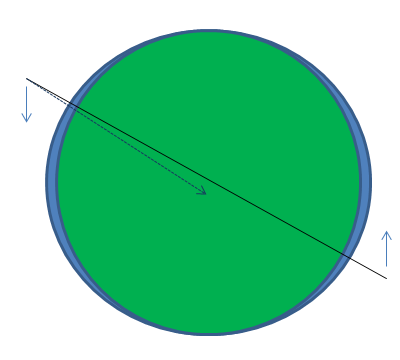
\includegraphics[scale=0.4]{Nodal_precession}
	\caption{From Wikipedia Nodal Precession}
\end{figure}

Intuitively, it would appear that the torque would reduce the inclination of the orbit.However, due to the bulge, the gravitational force is not directed towards the center of the body, but rather is offset toward the equatorial plane. As such, it causes torque-induced gyroscopic precession which causes the ascending and descending nodes to drift with time. This phenomenon is called \boldindex{nodal precession}.

The effects of nodal precession on the ascending and descending nodes is expressed by
\begin{align*}
	\dfrac{d\omega}{dt} &= \dfrac{3}{2}\:J_2\dfrac{R_E^2}{p^2}\bar{n}\left(2 - \dfrac{5}{2}\sin^2(i)\right)\\
	\dfrac{d\Omega}{dt} &= -\dfrac{3}{2}\:J_2\dfrac{R_E^2}{p^2}\bar{n}\cos(i)
\end{align*}
where $p = a(1 - e^2)$ is the semi-latus rectum of the orbit, $\bar{n}=\sqrt{\mathstrut\dfrac{\mu_E}{a^3}}$ is the mean motion, $R_E$ is the radius of the Earth, and $J_2$ is the Earths second dynamic form factor.

The $J_2$ term is a result of an infinite series equation that describes the perturbation effects of a rotating planetary body on the gravity of a planet. Each term of the series is denoted as $J_n$, however the $J_2$ term is more than 1000 times larger than the other terms \citep{J2Pertur39:online}. This is why the $J_2$ effect is considered a relevant orbital perturbation for the evolution of an orbital debris cloud. For context, Earth's  $J_2$ term has a value of $0.108 \times 10^{-2}$ whereas its $J_3$ term has a value of $0.253 \times 10^{-5}$.

\section{Analysis}

Now that the critical components for debris cloud evolution are established, we can use ODAP to gain insights into orbital debris's evolution. The first step is choosing a suitable scenario for the fragmentation event. Once the scenario is selected, the propagation methods defined in Section 4 can be applied to study the debris throughout the various phases. This includes analyzing the estimated time for the fragments to deorbit and the fragments' spread over time.

\subsection{Data Source}
Selecting a realistic scenario to analyze can be difficult without prior knowledge of typical satellite orbits. As such, it is beneficial to perform analysis on existing satellites in low Earth orbit. This can be accomplished by utilizing a database of \boldindex{Two-lines elements} (TLE's), which are a standardized way of describing information about a satellite's orbit.

ODAP utilizes a TLE database maintained by the website CelesTrak\footnote{Additional information about TLE's and CelesTrak can be found on their \href{URL}{https://www.celestrak.com/NORAD/elements/}} to make all cataloged objects in orbit available for fragmentation events.

The analysis conducted in the following subsections is performed on two different satellites. The first is a satellite called OXP 1, which has an altitude of approximately 750 km and a 25-degree inclination. This is in a higher region of low Earth orbit and will allow us to analyze long-term changes on the debris cloud.

The second satellite is a Starlink satellite produced by SpaceX. This satellite is at a much lower altitude, around 580 km, and is a member of a satellite mega constellation currently being constructed to provide global internet coverage. It was selected as part of this analysis due to the increasing number of companies expressing interest in low Earth orbit mega-constellations. Additionally, the Starlink mega-constellation is quickly grown to having over one thousand satellites in orbit, with the end goal being 30,000 (ADD SOURCE). It is relevant to study the debris cloud that would be produced in the case of a fragmentation event.

\subsection{Decay Time}

When a fragmentation event occurs, it is relevant to study the debris fragments' expected duration in orbit. Debris in orbit for a longer duration will have a higher probability of eventually colliding with other objects in space.

We expect that fragmentation events that occur in higher altitudes will generate debris that last longer. This is a direct consequence of drag's negligible effect at high altitudes due to the decreased air density. Additionally, since drag depends on the surface area of a debris fragment, we expect to see some debris fragments that deorbit faster than others at similar altitudes.

To analyze the orbital decay time using ODAP, we can use the simulated data from the band formation phase, where  perturbations. The output of this phase is the change in the Keplerian elements over time. As such, we can use the expression for the \boldindex{perigee}, which is the altitude at the lowest point of an orbit. The perigee is defined using Keplerian elements as
\begin{equation}
	z = a (1 - e).
\end{equation}
It should be noted that the perigee is being measured from the center of the Earth. To find the true altitude, we must subtract the radius of the Earth from the result.

Applying this process for both the Starlink satellite and OXP 1 results in the data used in Figure~\ref{altitudes}. The fragmentation event used in this simulation was identical for both satellites. The only changes were the starting orbits of the satellites. While only a random sample of data from both simulations is displayed in the Figure, the data revealed that 100\% of the Starlink fragments were deorbited within three years while only 1.5\% of the OXP 1 fragments were deorbited during this same interval.

This simulation concludes that fragmentation events occurring with mega-constellations in the lower region of LEO are of less concern than those occurring in higher orbits. While both create immense amounts of debris, the lower altitude Starlink satellites pose less of a threat to the long term health of LEO.

\begin{figure}[b!]
	\begin{adjustbox}{max width=1\linewidth,center}
		\centering     %%% not \center
		\subfigure[]{\label{fig:a}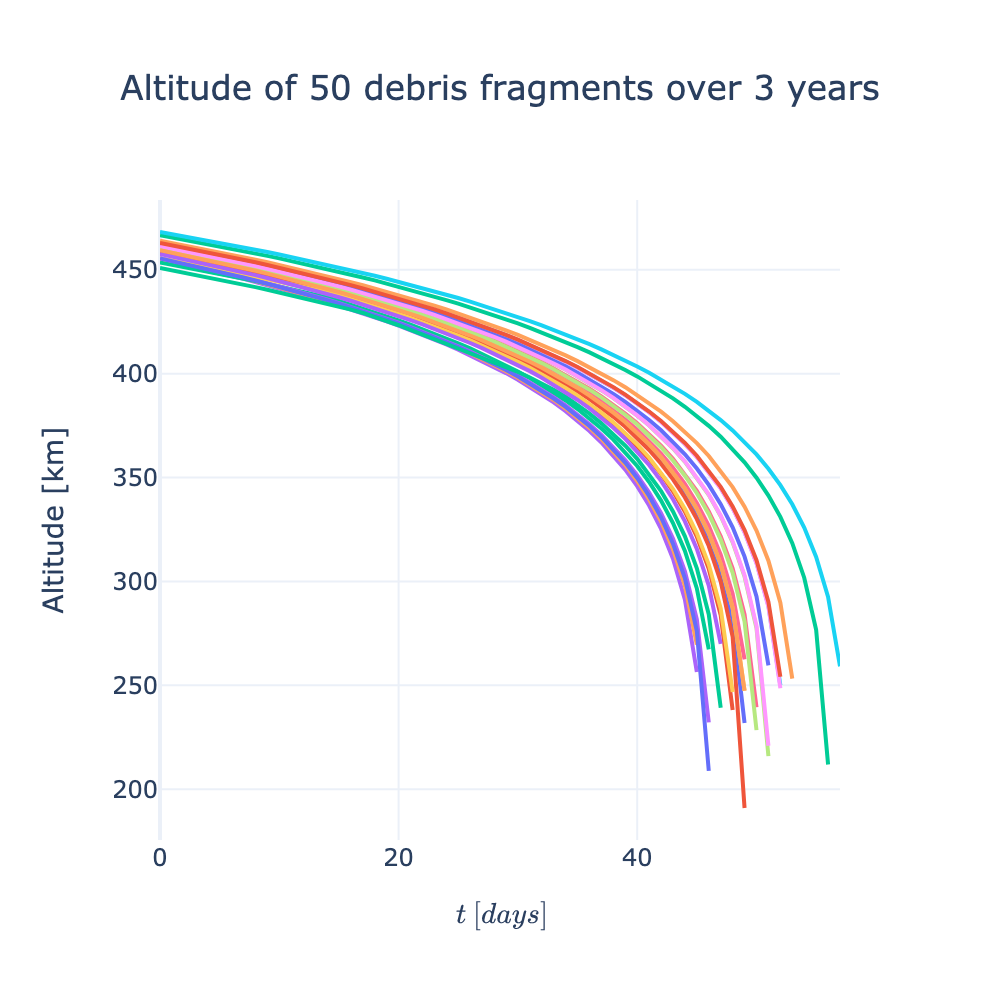
\includegraphics[width=0.5\textwidth]{Starlink_altitudes}}
		\subfigure[]{\label{fig:b}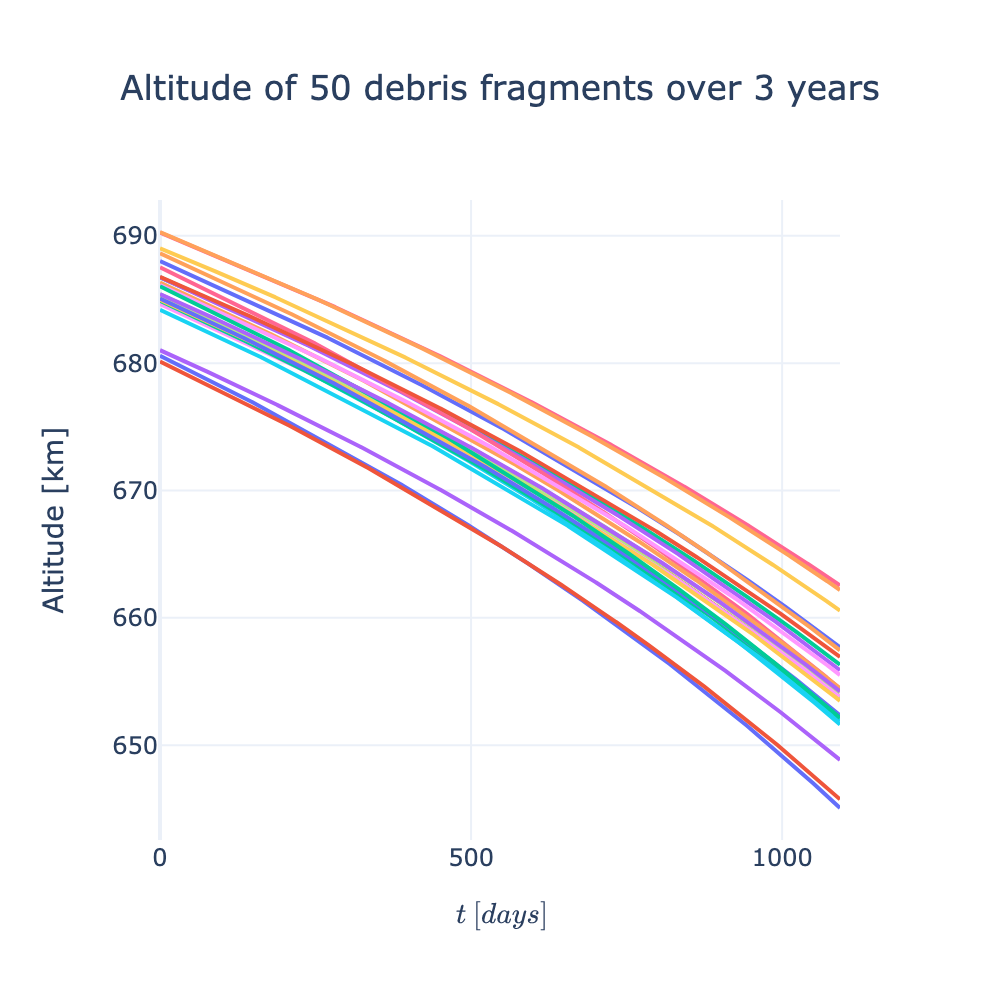
\includegraphics[width=0.5\textwidth]{oxp_altitudes}}
	\end{adjustbox}
	\caption{The altitudes of 50 pieces of debris generated by a non-catastrophic collision with a relative impact velocity of 2 km/s for both the Starlink satellite \textbf{(a)}, and OXP 1 \textbf{(b)} }
	\label{altitudes}
\end{figure}

\newpage
\subsection{Spread}
Another essential characteristic of orbital debris to study is the spread of the debris over time. The procedure for measuring the spread of the fragments performed similarly to the decay time. However, we do not need any additional equations and can visualize the spread of the fragments directly from the results provided by the band formation phase. We can use the distribution of the right angle of the ascending node $\Omega$ over time to get a sense of how the debris are spreading apart due to the $J_2$ perturbation.

This component of the analysis was conducted by performing a kernel density estimation on $\Omega$ at three different times of the band formation phase, the start, middle, and end time. A kernel density estimation is a way to estimate the probability density function of a random variable. As such, we can use it to get a sense of how the distribution of $\Omega$ changes throughout time. 

Figure~\ref{fig:starlink_dist} shows the results of performing this type of analysis on the fragmentation event used in the above subsection. As you can see, initially, most of the debris had a right angle of ascending node that was tightly clustered around the satellite's initial value. As the debris cloud evolves, this distribution becomes increasingly uniform. Notably, since the Starlink debris gets deorbited relatively quickly, it never has an opportunity to become entirely uniform. The simulated data for OXP exhibit this same phenomenon, thus allowing the analysis performed on the Starlink satellite suffice.

\newpage
In Section 5.2, we learned that the initial altitude of a breakup event dramatically impacts the time for the debris to deorbit. However, this Section revealed that it does not play a significant role in how spread out the debris becomes over time. The purpose of this analysis is to demonstrate how ODAP can be applied to gain new intuitions and understanding about the evolution of orbital debris.

\begin{figure}[t!]
	\centering
	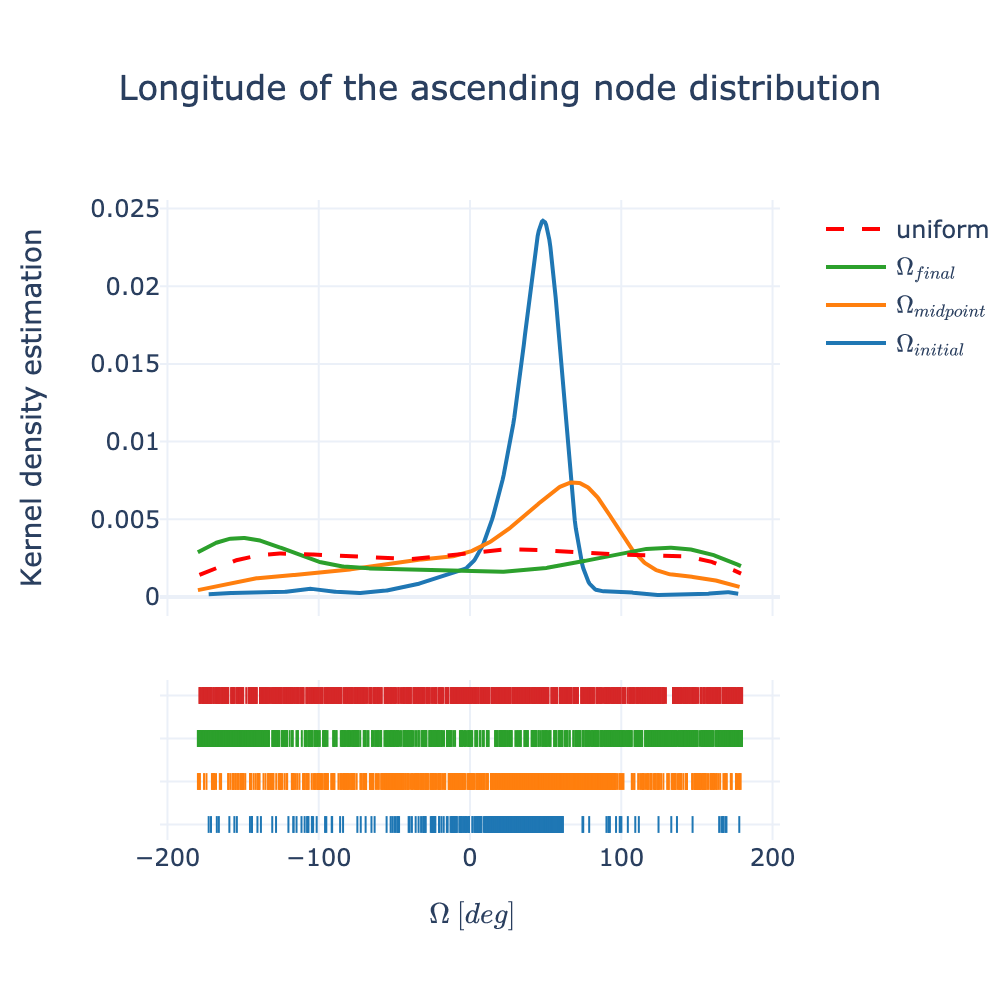
\includegraphics[scale=0.4, trim={0 0 0 2cm},clip]{starlink_dist}
	\caption{The kernel density estimation performed on the band formation phase of the Starlink satellite. The sampled values are from the beginning of the phase, the midpoint, and the end.}
	\label{fig:starlink_dist}
\end{figure}

\section{Conclusion}

Orbital debris will be a persistent problem as humankind continues to explore and utilize space to advance science. As such, the ability to model and study the effects associated with it is crucial. Unfortunately, much of the existing literature is difficult to find and gives an incomplete picture of the entire process needed to model orbital debris. Additionally, most of the available code to perform the analysis is written in older programming languages that are no longer widely used. Thus, ODAP was developed to be an open-source, easily accessible tool that utilizes a modern programming language to aid in research conducted in this field. This thesis also serves as a complete introduction to the necessary information needed to understand the process of modeling orbital debris.

There are many avenues for expanding on the research conducted in this thesis. One that I find most interesting is modeling the formed debris band analytically. This provides many benefits for conducting analysis but requires a significant amount of additional background information to understand. As such, it was outside the scope of this research. Additionally, refining ODAP to support different atmospheric models is a planned future addition. This would allow for a more in-depth analysis of the time it takes for debris to deorbit.

Many of these additional complexities are planned to be implemented into ODAP in the future. As such, the code base for ODAP is expected to evolve significantly over time. The appendix of this paper includes some of the most important functionality for reference, but the most up-to-date version will be found on Github.




%==========================================================================
%==========================================================================
% Appendices

\printindex

%\section{An other appendix}

%==========================================================================
%==========================================================================
% Bibliography.

% Some other possible styles: abbrv, acm, alpha, apalike, ieeetr, plain, siam, unsrt
\bibliographystyle{abbrvnat}
\bibliography{honors_thesis_bibliography} % Use the name of you bibliography file. Omit the ".bib" extension.

\newpage
\begin{appendices}
Write a description of what each section of the appendix covers
	
\section{Flux}

Let's pick a time interval T. Let's call N the number of debris pieces that cross the cross section (green plane in Figure xxx). Let's divide the time interval into M subinterval of length T/M.

What we measure in the simulation is the number debris crossing the cross section during each subinterval. What we're interested in predicting here is the statistics of those numbers when the positions of the debris along their orbits are distributed uniformly and independently from each other.

Each debris has a probability 1/M of crossing during a specific subinterval. The probability of exactly n debris crossing during a specific subinterval obeys a binomial distribution:

$$P_n = C_N^n \left(\frac{1}{M}\right)^n\left(1-\frac{1}{M}\right)^{N-n} . $$

Expectedly, the average number of debris crossing during a single subinterval is the number of debris crossing during the full interval (T) divided by the number of subintervals:

$$\left\langle P_n \right\rangle = \sum_0^N n P_n = \frac{N}{M} .$$

The variance is:

%$$\left\langle \left(P_n-\frac{N}{M}\right)^2 \right\rangle = ... = \frac{N}{M}\left(1-\frac{N}{M}\right) . $$
$$\left\langle \left(P_n-\langle P_n\rangle \right)^2 \right\rangle = ... = \frac{N}{M}\left(1-\frac{N}{M}\right) . $$

Therefore, if the debris ring is fully randomized and the average number of debris crossing per time step is $\phi$, we should expect the actual measurement to fluctate through time with a variance $\phi(1-\phi)$.

This in turn provides a criterion to assess whether the ring is fully randomized. Initially, when the debris are concentrated in a tight cluster, the variance is much higher. It then decreases gradually as the ring randomizes. When it becomes of order $\phi(1-\phi)$, we declare the ring randomized and move on to the band formation phase.

\section{Atm Model}
\begin{table}[h!]
	{
	\centering
	\begin{tabular}{lllll}\hline
		Lower Bound (km) & Upper Bound (km) & Base Altitude (km) & Nominal Density (kg/m\textasciicircum{}3) & Scale Height (km) \\ \hline
		0                         & 25                        & 0                  & 1.225E+00                                 & 7.249             \\ \hline
		25                        & 30                        & 25                 & 3.899E-02                                 & 6.349             \\ \hline
		30                        & 40                        & 30                 & 1.774E-02                                 & 6.682             \\ \hline
		40                        & 50                        & 40                 & 3.972E-03                                 & 7.554             \\ \hline
		50                        & 60                        & 50                 & 1.057E-03                                 & 8.382             \\ \hline
		60                        & 70                        & 60                 & 3.206E-04                                 & 7.714             \\ \hline
		70                        & 80                        & 70                 & 8.770E-05                                 & 6.549             \\ \hline
		80                        & 90                        & 80                 & 1.905E-05                                 & 5.799             \\ \hline
		90                        & 100                       & 90                 & 3.396E-06                                 & 5.382             \\ \hline
		100                       & 110                       & 100                & 5.297E-07                                 & 5.877             \\ \hline
		110                       & 120                       & 110                & 9.661E-08                                 & 7.263             \\ \hline
		120                       & 130                       & 120                & 2.438E-08                                 & 9.473             \\ \hline
		130                       & 140                       & 130                & 8.484E-09                                 & 12.636            \\ \hline
		140                       & 150                       & 140                & 3.845E-09                                 & 16.149            \\ \hline
		150                       & 180                       & 150                & 2.070E-09                                 & 22.523            \\ \hline
		180                       & 200                       & 180                & 5.464E-10                                 & 29.74             \\ \hline
		200                       & 250                       & 200                & 2.789E-10                                 & 37.105            \\ \hline
		250                       & 300                       & 250                & 7.248E-11                                 & 45.546            \\ \hline
		300                       & 350                       & 300                & 2.418E-11                                 & 53.628            \\ \hline
		350                       & 400                       & 350                & 9.518E-12                                 & 53.298            \\ \hline
		400                       & 450                       & 400                & 3.725E-12                                 & 58.515            \\ \hline
		450                       & 500                       & 450                & 1.585E-12                                 & 60.828            \\ \hline
		500                       & 600                       & 500                & 6.967E-13                                 & 63.822            \\ \hline
		600                       & 700                       & 600                & 1.454E-13                                 & 71.835            \\  \hline
		700                       & 800                       & 700                & 3.614E-14                                 & 88.667            \\ \hline
		800                       & 900                       & 800                & 1.170E-14                                 & 124.64            \\ \hline
		900                       & 1000                      & 900                & 5.245E-15                                 & 181.05            \\ \hline
		&                           &                    &                                           &                   \\
		&                           &                    &                                           &                   \\
		&                           &                    &                                           &                   \\
		&                           &                    &                                           &                  
	\end{tabular}
	}
\caption{Caption}
\label{atm}
\end{table}

%\section{Code}
%
%\subsection{Breakup Model}
%\label{subsec:breakup}
%\lstinputlisting[label = {alg:code/OrbitalDebris/generate_debris}, caption = {Perturbation Differential Equations Implementation}, firstline = 1, lastline = 378]
%{code/OrbitalDebris/generate_debris.py}
%
%\subsection{Coordinate Transforms}
%\label{subsec:transform}
%\lstinputlisting[label = {alg:code/OrbitalDebris/CoordTransforms}, caption = {Perturbation Differential Equations Implementation}, firstline = 1, lastline = 181]
%{code/OrbitalDebris/CoordTransforms.py}
%
%\subsection{Orbit Propagation}
%\label{subsec:propagation}
%\lstinputlisting[label = {alg:code/OrbitalDebris/Perturbations}, caption = {Perturbation Differential Equations Implementation}, firstline = 1, lastline = 255]
%{code/OrbitalDebris/Perturbations.py}
%
%
%\lstinputlisting[label = {alg:code/OrbitalDebris/Perturbations}, caption = {Perturbation Propagator}, firstline = 129, lastline = 156]
%{code/OrbitalDebris/Perturbations.py}
%
%	
	
\end{appendices}

\end{document}

